%-------------------------------------------------------------------------------
%                      Template Naskah Skripsi
%               	Berdasarkan format JTETI FT UGM
% 						(c) @gunturdputra 2014
%-------------------------------------------------------------------------------

%Template pembuatan naskah skripsi.
\documentclass{jtetiskripsi}

%Untuk prefiks pada daftar gambar dan tabel
\usepackage[titles]{tocloft}
\renewcommand\cftfigpresnum{Gambar\  }
\renewcommand\cfttabpresnum{Tabel\   }

%Untuk hyperlink dan table of content
\usepackage[hidelinks]{hyperref}
\newlength{\mylenf}
\settowidth{\mylenf}{\cftfigpresnum}
\setlength{\cftfignumwidth}{\dimexpr\mylenf+2em}
\setlength{\cfttabnumwidth}{\dimexpr\mylenf+2em}

%Untuk Bold Face pada Keterangan Gambar
\usepackage[labelfont=bf]{caption}

%Untuk caption dan subcaption
\usepackage{caption}
\usepackage{subcaption}

%pdf
\usepackage{pdfpages}

%table
\usepackage{array}
\usepackage{longtable}
\newcolumntype{P}[1]{>{\centering\arraybackslash}p{#1}}
\usepackage{graphics}
\usepackage{wrapfig}

%bibliography
\usepackage[
  style=authoryear-icomp,
  maxcitenames=1,
  isbn=false,
  doi=false,
  url=false,
  autolang=other,
  hyperref=true,
  sortcites=true,
  bibwarn=true,
  firstinits=true,
  autolang=other,
]{biblatex}
\DefineBibliographyStrings{english}{%
  andothers = {dkk\adddot,\addspace},
}
\DeclareFieldFormat{citehyperref}{%
  \DeclareFieldAlias{bibhyperref}{noformat}% Avoid nested links
  \bibhyperref{#1}}

\DeclareFieldFormat{textcitehyperref}{%
  \DeclareFieldAlias{bibhyperref}{noformat}% Avoid nested links
  \bibhyperref{%
    #1%
    \ifbool{cbx:parens}
      {\bibcloseparen\global\boolfalse{cbx:parens}}
      {}}}

\savebibmacro{cite}
\savebibmacro{textcite}

\renewbibmacro*{cite}{%
  \printtext[citehyperref]{%
    \restorebibmacro{cite}%
    \usebibmacro{cite}}}

\renewbibmacro*{textcite}{%
  \ifboolexpr{
    ( not test {\iffieldundef{prenote}} and
      test {\ifnumequal{\value{citecount}}{1}} )
    or
    ( not test {\iffieldundef{postnote}} and
      test {\ifnumequal{\value{citecount}}{\value{citetotal}}} )
  }
    {\DeclareFieldAlias{textcitehyperref}{noformat}}
    {}%
  \printtext[textcitehyperref]{%
    \restorebibmacro{textcite}%
    \usebibmacro{textcite}}}
\addbibresource{daftar-pustaka.bib}

%equation
\usepackage{amsmath}

%algorithm & syntax
\usepackage{algorithm}
\usepackage{algpseudocode}
\algnewcommand\algorithmicforeach{\textbf{for each:}}
\algnewcommand\ForEach{\item[ \algorithmicforeach]}
\algdef{SE}[DOWHILE]{Do}{doWhile}{\algorithmicdo}[1]{\algorithmicwhile\ #1}%
\newenvironment{conditions}
  {\par\vspace{\abovedisplayskip}\noindent\begin{tabular}{>{$}l<{$} @{${}={}$} l}}
  {\end{tabular}\par\vspace{\belowdisplayskip}}

%code
\usepackage{listings}
\usepackage{xcolor}
\definecolor{codegreen}{rgb}{0,0.6,0}
\definecolor{codegray}{rgb}{0.5,0.5,0.5}
\definecolor{codepurple}{rgb}{0.58,0,0.82}
\lstdefinestyle{mystyle}{
    commentstyle=\color{codegreen},
    keywordstyle=\color{magenta},
    numberstyle=\tiny\color{codegray},
    stringstyle=\color{codepurple},
    basicstyle=\ttfamily\footnotesize,
    frame=single,
    breakatwhitespace=false,
    breaklines=true,
    captionpos=b,
    keepspaces=true,
    numbersep=5pt,
    showspaces=false,
    showstringspaces=false,
    showtabs=false,
    tabsize=2
}
\lstset{style=mystyle}
\makeatletter
\def\thechapter{\@Roman\c@chapter}
\AtBeginDocument{%
  \def\thelstlisting{\@arabic\c@chapter.\@arabic\c@lstlisting}}
\makeatother


%-----------------------------------------------------------------
%Disini awal masukan untuk data proposal skripsi
%-----------------------------------------------------------------
\titleind{Penambahan Fungsi Indexing Pada Search Engine Telusuri Melalui
Inverted Index Untuk Meningkatkan Performa Waktu Pencarian}

\fullname{Mochammad Hanif Ramadhan}

\idnum{1313619025}

\approvaldate{23 Juni 2023}

\degree{Sarjana Ilmu Komputer}

\yearsubmit{2023}

\program{Ilmu Komputer}

\dept{Ilmu Komputer}

\firstsupervisor{Muhammad Eka Suryana, M. Kom.}
\firstnip{198512232012121002}

\secondsupervisor{Med Irzal, M. Kom.}
\secondnip{197706152003121001}

%-----------------------------------------------------------------
%Disini akhir masukan untuk data proposal skripsi
%-----------------------------------------------------------------

\tolerance=1
\emergencystretch=\maxdimen{}
\hyphenpenalty=10000
\hbadness=10000

\begin{document}

\cover{}
%-----------------------------------------------------------------

%-----------------------------------------------------------------
%Disini akhir masukan untuk muka skripsi
%-----------------------------------------------------------------

\chapter*{\centering{\large{LEMBAR PENGESAHAN}}}
\thispagestyle{empty} {\bf }Dengan ini saya mahasiswa Fakultas
Matematika dan Ilmu Pengetahuan Alam, Universitas Negeri Jakarta

\vskip3mm

\begin{tabular}{ll}
  Nama & : Prabowo Darmawi \\
  No. Registrasi & : 1313619001 \\
  Program Studi & : Ilmu Komputer \\
  Judul & : Penghitungan Panjang Dan Berat Ikan \\ & \hspace{0.2cm}
  Menggunakan Harris-Corners Detection \\
\end{tabular}

\vskip3mm

\noindent \hskip10mm Menyatakan bahwa proposal ini telah siap diajukan untuk seminar pra skripsi.
%\begin{center}
%Menyatakan bahwa skripsi ini telah siap diajukan untuk sidang skripsi.
%\end{center}



\begin{center}
\vskip3mm

Menyetujui,

\vskip3mm
\begin{spacing}{1.25}

\begin{tabular}{ccc}
  \hskip-2mm Dosen Pembimbing I & \qquad \qquad \qquad \qquad \qquad & \hskip-6mm Dosen Pembimbing II \\
   &  &  \\
   &  &  \\
   &  &  \\
   &  &  \\
  \hskip-2mm \underline{\textbf{Muhammad Eka Suryana, M.Kom}} &  & \hskip-6mm \underline{\textbf{Med
  Irzal, M.Kom}} \\
  \hskip-2mm NIP. 19770615 200312 1 001 &  & \hskip-6mm NIP. 19851223 201212 
  1 002	 \\
\end{tabular}
\end{spacing}
\end{center}
\vskip3mm
\begin{center}
Mengetahui, \\
Koordinator Program Studi Ilmu Komputer
\end{center}
\begin{spacing}{1.25}
{ \ }
\\
\\
{ \ }\begin{center}
\underline{\textbf{Dr. Ria Arafiyah, M.Si}} \\
{NIP. 19751121 200501 2 004}
\end{center}
\end{spacing} 

\chapter*{\centering{\large{KATA PENGANTAR}}}

Puji syukur penulis panjatkan ke hadirat Allah SWT, karena dengan rahmat dan
karunia-Nya, penulis dapat menyelesaikan proposal skripsi yang berjudul
\textit{Penghitungan Panjang dan Berat Ikan dengan Menggunakan Harris-Corner Detection}.

Keberhasilan dalam penyusunan proposal skripsi ini tidak lepas dari bantuan
berbagai pihak yang telah tulus dan ikhlas memberikan masukan guna sempurnanya proposal skripsi ini. Dalam kesempatan ini, dengan
kerendahan hati penulis mengucapkan banyak terima kasih kepada:

\begin{enumerate}

	\item{Yth. Para petinggi di lingkungan FMIPA Universitas Negeri Jakarta.}
	\item{Yth. Ibu Dr. Ria Arafiyah, M.Si selaku Koordinator Program Studi Ilmu
		Komputer.}
	\item{Yth. Bapak Muhammad Eka Suryana, M.Kom selaku Dosen Pembimbing I yang
		telah membimbing, mengarahkan, serta memberikan saran dan koreksi terhadap
		proposal skripsi ini.}
	\item{Yth. Bapak Med Irzal, M.Kom selaku Dosen Pembimbing II yang telah
		membimbing, mengarahkan, serta memberikan saran dan koreksi terhadap
		proposal skripsi ini.}
	\item{Kedua orang tua dan adik penulis yang telah mendukung dan memberikan 
		semangat serta doa untuk penulis.}
	\item{Teman-teman Program Studi Ilmu Komputer 2019 yang telah memberikan 
		dukungan dan memiliki andil dalam penulisan proposal skripsi ini.}
	
\end{enumerate}

Penulis menyadari bahwa penyusunan proposal skripsi ini masih jauh dari sempurna
karena keterbatasan ilmu dan pengalaman yang dimiliki. Oleh karenanya, kritik
dan saran yang bersifat membangun akan penulis terima dengan senang hati. 

Akhir kata, penulis berharap tugas akhir ini bisa bermanfaat bagi semua pihak baik itu bagi FMIPA Universitas Negeri Jakarta, teman-teman dari program studi Ilmu
Komputer Universitas Negeri Jakarta dan para pembaca sekalian, khususnya penulis sendiri.

Semoga Allah SWT senantiasa membalas kebaikan semua pihak yang telah membantu penulis dalam menyelesaikan proposal skripsi ini.

\vspace{4cm}

\begin{tabular}{p{7.5cm}c}
	&Jakarta, \\
	&\\
	&\\
	&\\
	&Prabowo Darmawi
\end{tabular}

\singlespacing{}
\tableofcontents{}
\addcontentsline{toc}{chapter}{DAFTAR ISI}
\listoffigures{}
\addcontentsline{toc}{chapter}{DAFTAR GAMBAR}
\listoftables{}
\addcontentsline{toc}{chapter}{DAFTAR TABEL}

\begin{counterpage}
\end{counterpage}
%Disini awal masukan untuk Bab
%-----------------------------------------------------------------
%!TEX root = ./template-skripsi.tex
%-------------------------------------------------------------------------------
% 								BAB I
% 							LATAR BELAKANG
%-------------------------------------------------------------------------------

\chapter{PENDAHULUAN}

\section{Latar Belakang Masalah}

Indonesia merupakan negara kepulauan dengan kekayaan hayati yang melimpah, salah satunya adalah ikan yang menjadi sumber pangan utama masyarakat. Budidaya ikan di Indonesia terus berkembang untuk memenuhi kebutuhan konsumsi dan permintaan pasar, baik sebagai bahan pangan maupun ikan hias. Salah satu aspek penting dalam budidaya ikan adalah pengukuran panjang dan berat ikan, yang berperan dalam pemantauan pertumbuhan, penentuan dosis pakan, serta penentuan harga jual.

Namun, proses pengukuran panjang dan berat ikan di lapangan umumnya masih dilakukan secara manual, yaitu dengan menimbang dan mengukur satu per satu menggunakan alat ukur konvensional (\cite{Amri2020}). Cara ini tidak efisien, memakan waktu lama, dan berpotensi menimbulkan stres pada ikan sehingga dapat mempengaruhi kualitas dan pertumbuhan ikan. Selain itu, metode manual hanya memberikan estimasi jumlah atau berat secara keseluruhan, tanpa informasi detail mengenai distribusi ukuran ikan dalam satu populasi.

Seiring perkembangan teknologi, pengolahan citra digital menawarkan solusi otomatis untuk mengukur panjang dan berat ikan secara cepat dan akurat. Salah satu metode yang dapat digunakan adalah deteksi titik sudut (\emph{corner detection}) pada citra ikan. Titik sudut pada tubuh ikan, seperti ujung kepala dan ekor, dapat digunakan sebagai acuan untuk mengukur panjang ikan secara otomatis dari citra (\cite{Harris2013}). Dengan mengetahui panjang ikan, berat ikan juga dapat diestimasi menggunakan rumus atau model regresi yang sesuai (\cite{Diansari2013}).

Metode \emph{Harris-Corner Detection} merupakan salah satu algoritma deteksi sudut yang banyak digunakan karena kestabilannya terhadap rotasi, noise, dan efisiensi komputasi (\cite{Harris2013}). Dengan menerapkan metode ini pada citra ikan, sistem dapat secara otomatis mendeteksi titik-titik sudut penting, sehingga proses pengukuran panjang dan estimasi berat ikan dapat dilakukan secara digital, cepat, dan minim kontak langsung dengan ikan.

Berbagai penelitian sebelumnya telah mengembangkan metode untuk mendeteksi atau melacak ikan, seperti penggunaan metode GMM dan Kalman Filter untuk pelacakan gerakan (Alim, 2021), serta GrabCut untuk pemisahan objek dari latar belakang (Nugraha, 2022). Namun, metode-metode tersebut umumnya hanya fokus pada deteksi keberadaan ikan atau pelacakan pergerakan, dan belum secara langsung mengekstraksi fitur geometris seperti panjang dan berat ikan.

Di sisi lain, metode seperti SIFT (\emph{Scale Invariant Feature Transform}) (\cite{Lowe2004}) memang kuat terhadap perubahan skala dan rotasi, namun proses perhitungannya relatif kompleks dan memerlukan waktu komputasi lebih tinggi. Untuk kasus estimasi bentuk linear seperti panjang dan lebar, pendekatan berbasis deteksi sudut seperti \emph{Harris-Corner Detection} terbukti lebih efisien dan akurat dalam mendeteksi titik-titik sudut penting pada citra (\cite{Harris2013}). \emph{Harris-Corner Detection} memberikan kestabilan terhadap rotasi dan noise lokal serta memiliki struktur komputasi yang lebih ringan dibanding SIFT, sehingga cocok untuk diterapkan dalam sistem real-time atau perangkat keras terbatas.

Oleh karena itu, penelitian ini bertujuan untuk membangun sistem pengukuran panjang dan estimasi berat ikan berbasis citra digital menggunakan metode \emph{Harris-Corner Detection}. Diharapkan sistem ini dapat membantu pembudidaya ikan dalam melakukan monitoring pertumbuhan ikan secara efisien dan akurat, serta mendukung pengambilan keputusan dalam manajemen budidaya.

\section{Rumusan Masalah}
Berdasarkan pemaparan masalah di atas, perumusan masalah dalam penelitian ini adalah \textbf{“Bagaimana cara mengukur panjang serta menghitung berat ikan menggunakan metode \emph{Harris-Corner Detection}?”}

\section{Batasan Masalah}
\begin{enumerate}
	\item Sistem hanya menghitung panjang dan berat ikan dengan menggunakan \emph{Harris-Corners Detection}. 
	\item Jenis Ikan yang digunakan adalah ikan lele, ikan mas, dan ikan nila.
	\item Sumber gambar berupa dataset yang diambil langsung dari lapangan.
	\item Dataset telah dihilangkan latar belakangnya dan digantikan dengan warna solid hitam.
	\item Citra yang digunakan hanya citra tampak samping. 
	\item Bahasa Pemrograman menggunakan Python 3 atau lebih baru. 
\end{enumerate}
	
\section{Tujuan Penelitian}
	Tujuan dari Penelitian adalah Membangun sistem berbasis citra digital untuk mengestimasi panjang dan berat ikan menggunakan deteksi titik sudut dengan menggunakan metode \emph{Harris-corner detection}. 

\section{Manfaat Penelitian}
\begin{enumerate}
	\item Bagi penulis
	 Memperoleh gelar sarjana dalam bidang Ilmu Komputer, dan menambah pengalaman dalam pembangunan sebuah sistem komputer untuk aplikasi dunia nyata, serta pengetahuan tentang pendeteksian sudut atau \emph{corner} dari \emph{Harris-corner Detection}. 

		
	\item Bagi Program Studi Ilmu Komputer
	Penelitian "Penghitungan Panjang dan Berat Ikan Menggunakan Harris-Corners Detection" dapat dijadikan sebagai referensi dan menambah wawasan mahasiswa dan sivitas akademika Ilmu Komputer Universitas Negeri Jakarta.

\end{enumerate}

% Baris ini digunakan untuk membantu dalam melakukan sitasi
% Karena diapit dengan comment, maka baris ini akan diabaikan
% oleh compiler LaTeX.
\begin{comment}
\bibliography{daftar-pustaka}
\end{comment}

%!TEX root = ./template-skripsi.tex
%-------------------------------------------------------------------------------
%                            BAB II
%                          KAJIAN TEORI
%-------------------------------------------------------------------------------

\chapter{KAJIAN PUSTAKA}

\section{\textbf{Multi-scale representation}}

Pada bagian ini akan dijelaskan representasi citra multi-resolusi berdasarkan filter Gaussian. 
Turunan Gaussian sering digunakan untuk mengekstrak fitur-fitur karakteristik. Bagian ini akan menjelaskan bagaimana menghitung stabilitas 
suatu gambar dan cara mengnormalisasi gambar tersebut untuk mendapatkan respons turunan yang tidak tergantung pada resolusi. 
Fitur lokal didefinisikan berdasarkan lokasi, skala, dan bentuk, yang akan mengalami transformasi saat dilihat dari sudut yang berbeda. 
Untuk memperkirakan perubahan transformasi pada suatu titik penting, kita dapat mengeksplorasi sifat dari \emph{Second moment matrix}, 
dengan komponen dari matriks Hessian digunakan untuk mendeteksi karakteristik skala struktur lokal dan mendeskripsikan bentuk struktur.

\subsection{\textbf{Gaussian scale-space}}

Dalam domain diskrit dari gambar digital, parameter skala juga diambil dalam bentuk diskrit. 
Sebagai hasilnya, representasi ruang-skala adalah kumpulan gambar yang direpresentasikan pada tingkat resolusi diskrit yang berbeda. 
Banyak penelitian dalam konteks skala-ruang menunjukkan bahwa salah satu persyaratan penting adalah bahwa representasi skala-ruang harus memenuhi persamaan yang dapat dicapai dengan melakukan konvolusi menggunakan kernel Gaussian. 
Selanjutnya, penelitian ini mengindikasikan bahwa kernel Gaussian adalah satu-satunya kernel yang unik yang dapat menghasilkan representasi skala-ruang. 
Keunikan dari kernel Gaussian ini telah dikonfirmasi melalui berbagai formulasi dalam berbagai penelitian lain. 
Temuan ini menyimpulkan bahwa konvolusi dengan kernel Gaussian merupakan solusi optimal untuk permasalahan konstruksi representasi skala-ganda. 
Fungsi Gaussian dua dimensi didefinisikan sebagai berikut:

\begin{equation*}
g(\sigma) = \frac{1}{2\pi\sigma^2}\exp^-\frac{x^2+y^2}{2\sigma^2}
\end{equation*}

Keunikan dari gaussian kernel dapat diketahui dari beberapa property berikut : 
\emph{linearity, separability, causality, and semi group property.} Keterpisahan 
atau \emph{separability} memungkinan \emph{multi-dimensional gaussian kernel} 
untuk diperoleh sebagai produk satu dimensi kernel : 

\begin{equation*}
  g(x,y) = g(x)g(y)
\end{equation*}

Properti ini memiliki kegunaan yang sangat signifikan dalam praktiknya karena penghalusan sinyal dua dimensi 
dapat digantikan oleh dua penghalusan satu dimensi, satu untuk setiap dimensi. 
Filter Gaussian satu dimensi dapat diimplementasikan sebagai filter rekursif, yang secara signifikan mempercepat proses 
perhitungan terutama pada kasus kernel Gaussian yang lebih besar (yaitu > \( \sqrt{2}\)). 
Kondisi kausalitas menyatakan bahwa tidak ada struktur buatan tambahan yang perlu dibuat saat menghitung citra dalam skala kasar, 
yang berarti citra pada skala yang lebih kasar merupakan representasi yang disederhanakan dari citra pada skala yang lebih halus. 
Sifat semi-grup komutatif menyatakan bahwa pemulusan sebanyak n kali pada sebuah gambar menghasilkan hasil yang sama dengan pemulusan satu kali 
menggunakan kernel dengan ukuran yang sama dengan jumlah seluruh n kernel yang digunakan. 
Selain itu, operasi n dapat dilakukan dalam urutan apa pun:

\begin{equation*}
g(\sigma_{1}) * \cdot * g(\sigma_{n}) * I(x) = g(\sigma_{1} + \cdot + \sigma_{n}) * I(x)
\end{equation*}

Biasanya, ruang-skala yang seragam digunakan, tetapi representasi ruang-skala umum dihitung dengan filter-filter lain.

\textbf{Uniform scale-space}. Perbeddan tingkat pada representasi skala-ruang
secara umum, terbuat dari konvolusi dengan \emph{gaussian kernel} :

\begin{equation*}
L(x,\sigma) = g(\sigma) * I(x)
\end{equation*}

Dengan I adalah gambar dan \(x = (x,y)\) adalah lokasi poin.
\emph{Kernel} adalah simetris sirkular dan diparameterisasi dari satu skala faktor \(\sigma \).

\begin{figure}
  \centering{}
  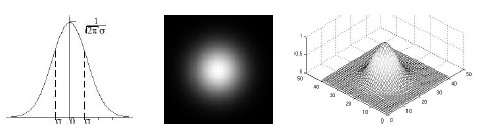
\includegraphics[width=0.8\textwidth]{gambar/Uniform Gaussian kernel.jpg}
  \caption{}
\end{figure}

Citra dalam skala kasar diperoleh dengan menghaluskan citra dalam skala halus. 
Proses ini diulangi secara berurutan pada tingkat skala yang semakin kasar untuk menghasilkan representasi multiskala. 
Untuk mempercepat operasi ini, seringkali dilakukan pengambilan sampel pada citra skala kasar dengan faktor skala yang sesuai setelah setiap operasi pemulusan. 
Namun, perlu berhati-hati dalam memilih skala dan faktor pengambilan sampel karena hal ini dapat menyebabkan masalah aliasing. 
Selain itu, diperlukan penambahan hubungan tambahan untuk mencocokkan lokasi titik yang sesuai pada tingkat skala yang berbeda. 
Ini membuat analisis teoretis menjadi lebih kompleks.

Alternatifnya, representasi skala-ruang juga dapat dibangun dengan meratakan gambar beresolusi tinggi secara berturut-turut dengan menggunakan kernel berbagai skala. 
Memang, membangun ruang-skala ini memerlukan lebih banyak waktu, terutama ketika tidak ada pengambilan sampel. 
Walaupun informasi menjadi redundant, namun tidak perlu menghitung lokasi titik yang sesuai pada setiap tingkat skala. 
Jika semua titik tetap dipertahankan pada setiap tingkat ruang-skala, maka hubungan antara analisis teoretis dan komputasi praktis tetap terjaga.

Detektor fitur, pada dasarnya, bergantung pada struktur sederhana seperti tensor matriks momen kedua dalam deteksi titik penting. 
Skala kepentingan dalam dan luar, yaitu di mana struktur dapat dianalisis, ditentukan oleh kondisi akuisisi, yaitu resolusi dan lapangan pandang. 
Ukuran minimal sebuah struktur gambar yang dapat dianggap sebagai karakteristik dibatasi oleh resolusi dan noise. 
Inner scale adalah faktor yang berhubungan dengan ukuran struktur tersebut, dengan kata lain, ukuran minimal lingkungan titik yang mengandung informasi penting tentang struktur. Outer scale, yang merupakan ukuran terbesar dari struktur, dibatasi oleh kendala yang menentukan sifat lokal dari fitur tersebut dan juga dibatasi oleh ukuran gambar itu sendiri. 
Faktor skala harus didistribusikan secara eksponensial antara batas dalam dan luar, yaitu \(\sigma_{n} = \sigma_{0}s^{n}\), 
agar perubahan informasi tetap seragam antara tingkat resolusi yang berurutan. 

\textbf{Affine scale-space.} Representasi yang lebih umum adalah ruang-skala affine. 
Teori ruang-skala affine Gaussian sangat bermanfaat ketika berurusan dengan transformasi yang halus dari bagian citra. 
Representasi ini dapat dihasilkan melalui konvolusi dengan kernel affine Gaussian.

\begin{equation}
  g(\Sigma) = \frac{1}{2\pi\sqrt{\det\Sigma}}\exp^{-\frac{x^{T}\Sigma^{-1}x}{2}}
\end{equation}

\begin{figure}
  \centering{}
  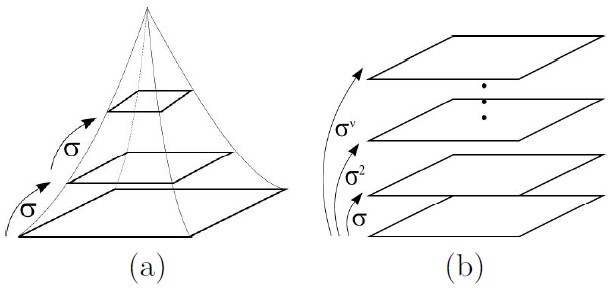
\includegraphics[width=0.8\textwidth]{gambar/Scale space.jpg}
  \caption{}
\end{figure}

\begin{figure}
  \centering{}
  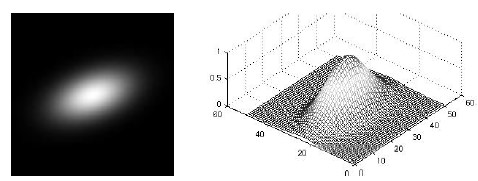
\includegraphics[width=0.8\textwidth]{gambar/Affine Gaussian kernel.jpg}
  \caption{}
\end{figure}

Jika matriks \(\Sigma\) adalah matriks identitas dikalikan dengan skalar, 
maka fungsi ini sesuai dengan Kernel Gaussian Uniform. Penulis mengatasi ruang tiga dimensi (x, y, \(\sigma\)) 
jika menggunakan pendekatan tradisional, di mana filter Gaussian seragam digunakan. 
Kernel Gaussian dalam hal ini ditentukan oleh satu parameter skala, yaitu \(\sigma\). 

Namun, ketika matriks \(\Sigma\) adalah matriks positif simetris 2x2, 
kompleksitasnya menjadi lebih tinggi karena kita berada dalam ruang berdimensi tinggi yang sulit dihandle. 
Meskipun begitu, kompleksitas ini dapat dikelola jika kita hanya menghitung representasi untuk satu titik citra. 
Filter affine yang diterapkan pada titik tertentu biasanya digunakan untuk masalah bentuk-dari-tekstur.

Ada beberapa pendekatan untuk menghitung konvolusi dengan kernel affine. 
Salah satu pendekatan adalah dengan menggunakan transformasi Fourier dari kernel Gaussian diskrit dan melakukan perkalian dengan citra dalam domain frekuensi. 
Jika hanya perlu menghitung respons filter pada satu titik citra, tidak ada manfaat dalam menggunakan filter rekursif. 
Biaya komputasi yang sama akan diperoleh dengan mengambil sampel kernel affine dan langsung menggabungkannya dengan citra. 

Metode yang digunakan dalam pendekatan yang dijelaskan dalam manuskrip ini didasarkan pada dekomposisi matriks kernel menjadi produk rotasi dan penskalaan matriks.


\begin{equation*}
\Sigma = R^{T} \cdot D \cdot R =  
\begin{bmatrix} 
\cos (\phi )&  -\sin (\phi) \\ 
\sin (\phi )& \cos (\phi) 
\end{bmatrix} 
\begin{bmatrix}
\sigma_{x} &0 \\
0 & \sigma_{y}
\end{bmatrix}
\begin{bmatrix}
\cos (\phi )&  \sin (\phi) \\ 
-\sin (\phi )& \cos (\phi)
\end{bmatrix}
\end{equation*}

Persamaan ini menunjukkan bahwa pemulusan affine setara dengan melakukan konvolusi dengan kernel Gaussian yang telah dirotasi dan memiliki bentuk elips. 
Untuk menyederhanakan proses komputasi, kita dapat melakukan perubahan pada titik:

\begin{equation*}
x^{T}\Sigma^{-1}x = x^{T}\frac{1}{\sigma_{x}\sigma_{y}}\Sigma^{-1}_{N}x=x^{T}\Sigma^{-\frac{1}{2}}_{N}\frac{1}{\sigma_{x}\sigma_{y}}\Sigma^{-\frac{1}{2}}_{N}x=(\Sigma^{-\frac{1}{2}}_{N}x)^{T}\frac{1}{\sigma_{x}\sigma_{y}}\Sigma^{-\frac{1}{2}}_{N}x
\end{equation*}

Dengan demikian, pemulusan affine dilakukan dengan melakukan konvolusi menggunakan kernel seragam \(\sigma_{N} = \sqrt{\sigma_{x}\sigma_{y}}\)
dengan titik yang ditransformasi oleh \(x' = \Sigma^{1\frac{1}{2}}_{N}x\). Sebuah masalah terjadi ketika \(\sigma_{x}\) 
sangat berbeda dari \(\sigma_{y}\). Dalam hal ini, pengambilan sampel citra dilakukan dengan interval \(\frac{\sigma_{x}}{\sigma_{N}}\)
dan \(\frac{\sigma_{y}}{\sigma_{N}}\) melibatkan beberapa kehilangan informasi dan mengenalkan artefak. 
Mengatasi masalah ini dapat mengatur ukuran kernel yang seragam untuk \(\sigma_{N} = \max(\sigma_{x},\sigma_{y})\)
dan kemudian menghitung matriks \(\Sigma^{-\frac{1}{2}}_{N}\). 

\begin{figure}
  \centering{}
  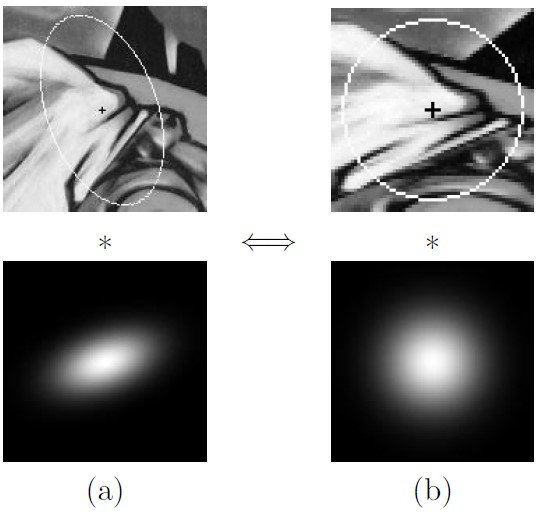
\includegraphics[width=0.8\textwidth]{gambar/Smoothing gaussian kernel.jpg}
  \caption{}
\end{figure}

\subsection{\textbf{Scale-space derivatives}}

Kegunaan turunan dalam analisis sinyal lokal dapat diilustrasikan melalui ekspansi Taylor. 
Ekspansi Taylor memegang peran penting dalam desain filter dan, pada urutan yang dipilih, mendekati struktur gambar secara lokal. 
Secara umum, ekspansi ini dihitung hingga urutan kedua.

\begin{equation*}
  I(x_{0} +\Delta x) \approx I(x_{0}) + \Delta x^{T}\nabla  I(x_{0}) + \Delta x^{T} H(x_{0}) \Delta x
\end{equation*}

\textbf{Gaussian derivatives} Sebuah fitur dapat diekstrak pada berbagai tingkat resolusi dengan menerapkan fungsi yang sesuai pada skala yang berbeda. 
Fungsi deteksi banyak didasarkan pada turunan Gaussian dalam ruang-skala, karena turunan Gaussian linear cocok untuk memodelkan pemrosesan visual dalam manusia. 
Perbedaan besar ini, yang dihitung dengan menggabungkan sinyal asli dengan turunan dari Gaussian, dapat dianggap sebagai generalisasi operator perbedaan. 
Ketika parameter skala mendekati nol, turunan dalam ruang-skala mendekati turunan dari fungsi asli. 
Tujuan dari analisis dalam ruang-skala adalah untuk menyelidiki representasi citra pada berbagai tingkat skala guna mengekstrak informasi yang signifikan.

\textbf{Uniform derivatives} Secara umum, dalam praktik pemrosesan citra, filter yang berasal dari kernel Gaussian seragam sering digunakan. 
Turunan pada berbagai tingkat skala dapat dihitung dengan menghaluskan citra menggunakan filter Gaussian dan kemudian menghitung perbedaannya. 
Semua properti yang berlaku untuk kernel Gaussian juga berlaku untuk turunannya. Oleh karena itu, jika kita menerapkan operasi ini dalam urutan terbalik, 
kita akan mendapatkan hasil yang sama. Alternatifnya, kita juga dapat menggabungkan citra dengan turunan dari kernel Gaussian pada berbagai skala. 
Semua metode ini bersifat setara. Dalam hal ini, untuk setiap fungsi citra \(I(x)\), turunan pertama dapat didefinisikan sebagai berikut:

\begin{equation*}
  L_{x}(x;\Sigma) = \frac{\partial}{\partial_{x}} * g(\Sigma) * I(x)
\end{equation*}

Persamaan umum untuk turunan Gauss adalah sebagai berikut:

\begin{equation*}
  g_{i_{1}\cdots i_{m}}(x,\Sigma) =\frac{\partial}{\partial_{i_{1}}\cdots \partial_{i_{m}}}\frac{1}{2\pi\sqrt{\det}}\exp^{-\frac{x^{T}\Sigma^{-1}x}{2}}
\end{equation*}

di mana \(m\) adalah urutan turunan dan \(i\) adalah koordinat Cartesian pada gambar. 
Dalam kasus ketika \(\Sigma\) adalah matriks identitas yang dikalikan dengan skalar, maka akan 
berurusan dengan turunan Gaussian seragam tradisional. 

\textbf{Normalized derivatives} Amplitudo turunan spasial, secara umum, berkurang dengan skala, 
karena responsnya lebih halus pada skala yang lebih besar. Dalam kasus struktur yang ada pada rentang 
skala besar, seperti \emph{corner} atau \emph{step-edge}, dan berharap memiliki konstanta turunan 
atas skala. Untuk menjaga properti \emph{Scale invariance}, fungsi turunan harus dinormalisasi 
sehubungan dengan skala turunan.Turunan \(D\) yang dinormalisasi skala dari orde \(m\) didefinisikan oleh:

\begin{equation*}
  D_{i_{1}\cdots i_{m}}(x,\sigma) = \sigma^{m}L_{i_{1} \cdot i_{m}}(x,\sigma) = \sigma^{m}g_{i_{1}\cdot i_{m}}(\sigma)*I(x)
\end{equation*}

persamaan berikut menunjukkan perlunya menggunakan faktor normalisasi \(\sigma^{m}\). 
Pertimbangkan dua citra \(I\) dan \(I'\) yang dicitrakan pada skala yang berbeda.
Relasi antara dua gambar tersebut kemudian didefinisikan dengan: \(I(x) = I'(x')\) , 
dimana \(x' = sx\). Perhatikan bahwa kemungkinan pergeseran suatu titik diabaikan, 
karena dihilangkan oleh diferensiasi. Derivatif gambar kemudian:

\begin{equation*}
  I_{i_{1}\cdot i_{m}}(x') = s^{m}I_{i_{1}\cdot i_{m}}(sx')
\end{equation*}

Jika menganggap bahwa kernel turunan dari skala \(\sigma\) dinormalisasi oleh 
faktor skala yang sama, maka memperoleh:

\begin{equation*}
  \sigma^{m}g_{i_{1}\cdot i_{m}}(\sigma) * I(x)= s^{m}\sigma^{m}g_{i_{1}\cdot i_{m}}(s\sigma)*I(x')
\end{equation*}

Jadi, untuk turunan yang dinormalisasi, responsnya memiliki nilai yang sama:

\begin{equation*}
  D_{i_{1}\cdot i_{m}}(x,\sigma) = D'_{i_{1}\cdot i_{m}}(x,s\sigma)
\end{equation*}

Dengan dapat melihat bahwa jika mengalikan turunan dengan ukuran kernel, 
dan memperoleh nilai turunan yang sama untuk struktur lokal yang direpresentasikan 
pada skala yang sesuai.

\begin{figure}
  \centering{}
  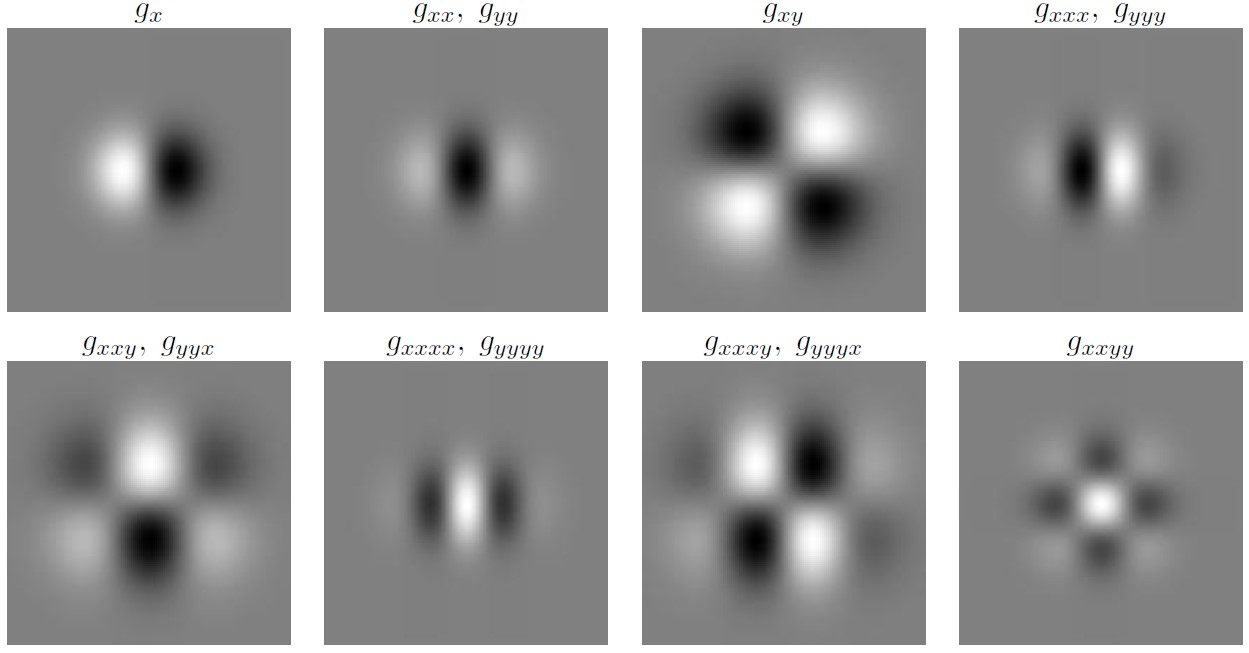
\includegraphics[width=0.8\textwidth]{gambar/Uniform Gaussian derivatives.jpg}
  \caption{}
\end{figure}

\textbf{Affine derivatives} Turunan affine sangat berguna jika berurusan dengan 
invarian affine. Untuk mendapatkan invarian affine dari turunan struktur lokal sembarang, 
kernel Gaussian harus disesuaikan dengan bentuk dan skala struktur. Dengan demikian bentuk 
anisotropik dari fitur tersebut tidak dibias oleh penghalusan isotropik dengan filter seragam. 
Untuk mengadaptasi filter, tanpa pengetahuan sebelumnya tentang bentuk struktur, diharus 
mengeksplorasi banyak kemungkinan kombinasi dari parameter kernel. Namun, tiga derajat kebebasan 
dari kernel affine Gaussian membuatnya sulit untuk menyelidiki semua kemungkinan kombinasi. 
Oleh karena itu, dalam praktiknya hanya dibatasi kemungkinan bentuk kernel saja. 
Komputasi turunan arah affine untuk semua titik citra dapat dipercepat dengan implementasi rekursif. 

\subsection{\textbf{Second moment matrix}}

\emph{Second Moment matrix} dijelaskan pada bagian ini sering digunakan untuk deteksi 
fitur atau deskripsi struktur citra lokal. Matriks ini disebut juga \emph{Auto-correlation Matrix} 
dan didefinisikan dengan:

\begin{equation}
  \mu(x,\sigma_{I},\sigma_{D})= 
  \begin{bmatrix}
   \mu_{11} & \mu_{12} \\
   \mu_{21} & \mu_{22} 
   \end{bmatrix} =
   \sigma^{2}_{D}g(\sigma_{I}) *
   \begin{bmatrix}
   L^{2}_{x}(x,\sigma_{D}) & L_{x}L_{y}(x,\sigma_{D}) \\
   L_{x}L_{y}(x,\sigma_{D}) & L^{2}_{y}(x,\sigma_{D}) 
   \end{bmatrix}
\end{equation}

Ini menjelaskan distribusi gradien di lingkungan lokal dari suatu titik. Derivatif gradien ditentukan 
oleh skala lokal \(\sigma_{D}\) (skala derivasi). Derivasi dirata-ratakan di sekitar titik dengan 
menghaluskan menggunakan jendela Gaussian berukuran \(\sigma_{I}\) (skala integrasi).
Nilai eigen dari matriks ini merepresentasikan dua kelengkungan utama dari suatu titik. 
Properti ini memungkinkan ekstraksi titik, yang kedua kelengkungannya signifikan, yaitu perubahan 
sinyal signifikan dalam arah ortogonal. Titik-titik ini lebih stabil dalam kondisi pencahayaan acak 
dan lebih representatif daripada titik gambar lainnya.
Dalam ruang-skala affine, \emph{Second moment matrix} \(\mu\) pada titik tertentu \(x\) didefinisikan oleh:

\begin{equation*}
  \mu(x, \Sigma_{I}, \Sigma_{D} ) = \det(\Sigma_{D})g(\Sigma_{I})* ((\nabla L)(x, \Sigma_{D})(\nabla L)(x, \Sigma_{D})^{T})
\end{equation*}

dimana \(\Sigma_{I}\) dan \(\Sigma_{D}\) adalah matriks kovarians yang menentukan integrasi dan 
derivasi kernel Gaussian. Dalam praktik tidak mungkin menghitung matriks untuk semua kemungkinan 
kombinasi parameter kernel. Untuk membatasi jumlah derajat kebebasan dengan menerapkan 
kondisi \(\Sigma_{I} = s\Sigma_{D}\), dimana \(s\) adalah skalar. Oleh karena itu, derivasi dan integrasi 
kernel akan berbeda hanya dalam ukuran dan bukan dalam bentuk. Ini berarti faktor skala antara dua arah ortogonal 
sama untuk menghaluskan dan mengintegrasikan turunan dari \emph{second moment matrix}.

\textbf{Affine transformation of a point} Matriks momen kedua memiliki sifat yang membuatnya sangat berguna 
untuk memperkirakan bentuk anisotropik dari struktur citra lokal. Pertimbangkan sebuah titik \(x_{L}\) yang 
diubah oleh transformasi linear \(x_{R} = Ax_{L}\). Matriks \(\mu_{L}\) yang dihitung pada titik \(x_{L}\) 
kemudian ditransformasikan dengan cara berikut:

\begin{equation}
  \mu(x_{L},\Sigma_{I,L},\Sigma_{D,L}) = A^{T}\mu(A_{xL},A\Sigma_{I,L}A^{T},A\Sigma_{D,L}A^{T})A = A^{T}\mu(x_{R},\Sigma_{I,R},\Sigma_{D,R})A
\end{equation}

Jika menunjukkan matriks yang sesuai dengan:

\begin{equation*}
  \mu(x_{L},\Sigma_{I,L},\Sigma_{D,L}) = M_{L} \quad \mu(x_{R},\Sigma_{I,R},\Sigma_{D,R}) = M_{R}
\end{equation*}


matriks-matriks tersebut kemudian dihubungkan dengan:

\begin{equation}
  M_{L} = A^{T}M_{R}A \quad M_{R} = A^{-T}M_{L}A^{-1}
\end{equation}

Derivasi dan kernel integrasi dalam hal ini diubah oleh:

\begin{equation*}
  \Sigma_{R} = A\Sigma_{L}A^{T}
\end{equation*}

Misalkan matriks \(M_{L}\) dihitung sedemikian rupa sehingga (Kondisi 1):

\begin{equation}
  \Sigma_{I,L}=\sigma_{I}M_{L}^{-1} \quad \Sigma_{D,L}=\sigma_{D}M_{L}^{-1}
\end{equation}

dimana skalar \(\sigma_{I}\) dan \(\sigma_{D}\) masing-masing adalah skala integrasi dan derivasi. 
Selanjutnya dapat menurunkannya sebagai berikut (Kondisi):

\begin{equation}
  \Sigma_{I,R} = A\Sigma_{I,L}A^{T} = \sigma_{I}(AM_{L}^{-1}A^{T}) = \sigma_{I}(A^{-T}M_{L}A^{-1})^{-1} = \sigma_{I}M_{R}^{-1} \\
  \Sigma_{D,R} = A\Sigma_{D,L}A^{T} = \sigma_{D}(AM_{L}^{-1}A^{T}) = \sigma_{D}(A^{-T}M_{L}A^{-1})^{-1} = \sigma_{D}M_{R}^{-1}
\end{equation}

Dapat dilihat bahwa memaksakan kondisi 1 memerlukan hubungan kondisi 2 dengan asumsi bahwa 
titik-titik tersebut terkait dengan transformasi affine. Sekarang dapat membalikkan masalahnya dan 
menganggap memiliki dua titik yang dihubungkan oleh transformasi affine yang tidak diketahui. 
Jika diestimasi matriks \(\Sigma_{R}\) dan \(\Sigma_{L}\) sehingga matriks tersebut memverifikasi 
kondisi 1 dan 2, maka relasi 3.4 benar. Properti yang disajikan memungkinkan parameter transformasi 
diekspresikan secara langsung oleh komponen matriks. Transformasi affine kemudian bisa didefinisikan oleh :

\begin{equation*}
  A = M_{R}^{-\frac{1}{2}}R M_{L}^{-\frac{1}{2}}
\end{equation*}

dimana \(R\) mewakili rotasi sewenang-wenang. Pada bab berikutnya akan disajikan algoritma iteratif untuk memperkirakan matriks \(\Sigma_{R}\) dan \(\Sigma_{L}\) dan 
bagaimana memulihkan rotasi \(R\) dengan cara yang kuat. Dengan demikian, dapat memperkirakan transformasi afin antara dua titik yang bersesuaian 
tanpa pengetahuan sebelumnya tentang transformasi ini. Selanjutnya, matriks \(M_{L}\) dan \(M_{R}\), dihitung pada kondisi 3.5 dan 3.6, menentukan daerah korespondensi 
yang didefinisikan oleh \(X^{T}M_{x}=1\). Jika ketetanggaan titik \(x_{R}\) dan \(x_{L}\) dinormalisasi dengan transformasi \(x'_{R}=M^{\frac{1}{2}}_{R}x_{R}\) dan \(x'_{L}=M^{\frac{1}{2}}_{L}x_{L}\), masing-masing, 
daerah yang dinormalisasi dihubungkan dengan rotasi sederhana \(x'_{L}=Rx'_{R}\)

\begin{equation}
  x_{R} = A x_{L} = M_{R}^{-\frac{1}{2}}R M_{L}^{\frac{1}{2}} x_{L}, \quad M_{R}^{\frac{1}{2}}x_{R} = R M_{L}^{\frac{1}{2}} x_{L}
\end{equation}

Matriks \(M'_{L}\) dan \(M'_{R}\) dalam bingkai yang dinormalisasi sama dengan matriks rotasi murni. Dengan kata lain, pola intensitas dalam bingkai yang dinormalisasi bersifat isotropik

\textbf{Isotropy measure} Berikut ini adalah menginterpretasikan \emph{second moment matrix}, yang disajikan 
di atas, dalam kaitannya dengan ukuran isotropi. Tanpa kehilangan keumuman, kami menganggap bahwa struktur 
anisotropik lokal adalah struktur isotropik yang ditransformasi \emph{affine}. Ini memberikan solusi untuk 
masalah deformasi affine pola lokal bila dilihat dari sudut yang berbeda. Struktur isotfropik yang 
dideformasi oleh transformasi affine menjadi anisotropik. Untuk mengimbangi deformasi affine, 
diharus menemukan transformasi yang membawa pola anisotropik ke isotropik. 
Perlu diperhatikan bahwa mempertahankan rotasi isotropi atau anisotropi dari patch citra.
Oleh karena itu, deformasi afin struktur isotropik dapat ditentukan hingga faktor rotasi. 
Faktor ini dapat dipulihkan dengan metode lain. \emph{second moment matrix} \(\mu(x,\sigma_{I},\sigma_{D})\)
dapat diartikan sebagai ukuran isotropi yang diterapkan pada titik \(x\) dalam lingkungan lokal berukuran \(\sigma_{I}\). 
Isotropi lokal dapat diukur oleh nilai eigen matriks \(\mu\). Jika nilai eigennya sama, dapat dianggap titik tersebut isotropik. 
Untuk memperoleh ukuran yang dinormalisasi penggunakan rasio nilai eigen:

\begin{equation}
  Q = \frac{\lambda_{min}(\mu)}{\lambda_{max}(\mu)}
\end{equation}

Nilai \(Q\) bervariasi dalam kisaran \(\left| 0 \cdots  1\right|\) dengan 1 untuk struktur isotropik yang sempurna. 
Pengukuran ini dapat memberikan respons yang sedikit berbeda untuk skala yang berbeda karena matriks \(\mu\) 
ditentukan oleh dua parameter skala. Skala-skala ini harus dipilih secara independen dari resolusi gambar.

Teknik pemilihan skala yang dijelaskan pada bagian berikutnya, memberikan kemungkinan untuk menentukan skala integrasi yang 
terkait dengan struktur citra lokal. Skala derivasi dan integrasi dapat dihubungkan dengan \(\sigma_{D}=s \sigma_{I}\), dengan \(s\) adalah 
faktor konstanta. Untuk alasan yang jelas skala derivasi harus selalu lebih kecil dari skala integrasi. Faktor s tidak boleh 
terlalu kecil, jika tidak smoothing terlalu signifikan terhadap derivasi. Di sisi lain \(s\) harus cukup kecil, sehingga \(\sigma_{I}\) dapat 
merata-ratakan matriks kovarians \(\mu(x,\sigma_{D},\sigma_{I})\) di lingkungan sekitar. Idenya adalah untuk menekan noise tanpa menekan bentuk 
anisotropik dari struktur gambar yang diamati. Pendekatan yang lebih canggih adalah memilih skala derivasi \(\sigma_{D}\) secara independen 
dari skala \(\sigma_{I}\) . Mengingat skala integrasi  dapat mencari skala \(\sigma_{D}\), dimana respon dari ukuran isotropi mencapai maksimum lokal. 
Dengan demikian, bentuk yang dipilih untuk struktur yang diamati kurang anisotropik. Pendekatan serupa untuk memilih skala lokal tetapi dia mengusulkan pemilihan skala yang anisotropinya dinormalisasi diasumsikan 
maksimum melebihi skala.

\begin{equation}
  Q_{A} = \frac{\sqrt{trace^{2}\mu - 4\det\mu}}{trace\mu}
\end{equation}

Ukuran ini juga dapat dinyatakan oleh nilai eigen:

\begin{equation*}
  Q_{A} = \left\lvert \frac{\lambda_{max}(\mu) - \lambda_{min}(\mu)}{\lambda_{max}(\mu) + \lambda_{min}(\mu)}\right\rvert 
\end{equation*}

Perhatikan kesamaan antara \(Q\) dan \(Q_{A}\). Meskipun, \(Q_{A}\) cenderung nol jika titiknya menjadi lebih isotropik. 
Berlawanan dengan pendekatan, pola gambar tidak dinormalisasi afin dalam prosedur iteratif yang memperkirakan bentuk anisotropik. 
Selanjutnya, dalam percobaan selanjutnya, melihat bahwa prosedur ini menyimpang lebih sering jika skala lokal dipilih dengan ukuran \(Q_{A}\) maksimum.

\section{\textbf{Automatic scale selection}}
Skala invariansi merupakan salah satu tujuan dalam pekerjaan ini, oleh karena itu pada bagian ini kami fokus 
pada metode untuk menentukan skala struktur citra lokal. Pemilihan skala otomatis dan sifat dari skala yang 
dipilih telah dipelajari secara ekstensif. Idenya adalah untuk memilih skala karakteristik, 
dimana fungsi tertentu mencapai skala ekstrem. Karakteristik nama sedikit arbitrer karena struktur lokal 
dapat eksis pada rentang skala dan dalam rentang ini tidak ada skala persepsi yang disukai. 
Namun, untuk deskriptor tertentu sebuah skala dapat diberi nama karakteristik, jika deskriptor yang 
dihitung pada skala ini dapat menyampaikan informasi lebih banyak dibandingkan dengan deskriptor pada skala lain.

\subsection{\textbf{Scale-space maxima}}
Berikut ini disajikan hubungan analitis antara skala maksimum ruang dan skala struktur citra lokal. 
Biarkan \(F\) menjadi fungsi yang dinormalisasi sehubungan dengan skala, yang digunakan untuk membangun ruang-skala. 
Himpunan respons untuk titik \(x\) kemudian ditentukan oleh \(F(x,\sigma_{n})\) dengan \(\sigma_{n} =\sigma_{0}s^{n}\). 
Himpunan ini disebut jejak skala. Faktor \(\sigma_{n}\) adalah skala awal pada tingkat resolusi terbaik dan \(\sigma_{n}\) 
menunjukkan tingkat representasi skala-ruang yang berurutan. Parameter memungkinkan peningkatan skala secara eksponensial untuk memperoleh 
perubahan informasi yang seragam antara level skala.

\begin{figure}
  \centering{}
  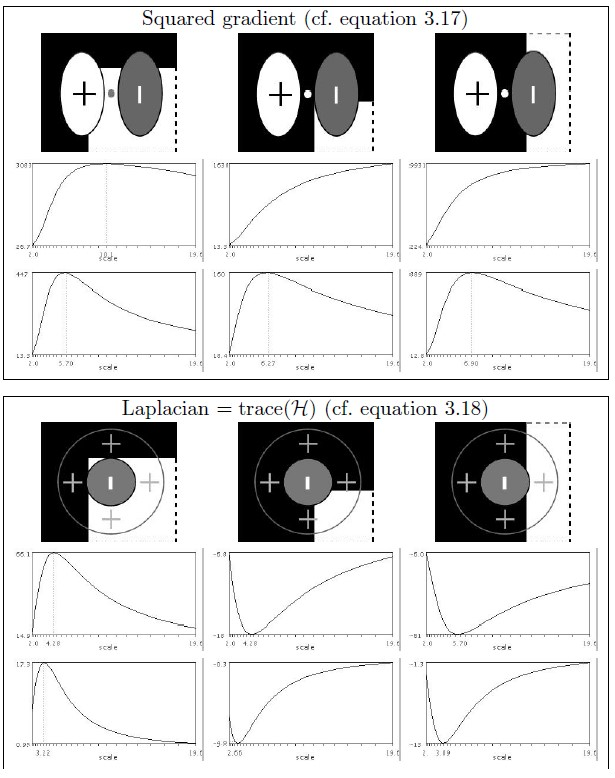
\includegraphics[width=0.8\textwidth]{gambar/Scale trace.jpg}
  \caption{\emph{Scale trace of squared gradient and Laplacian} diterapkan pada model sudut dan tepi. Kolom pertama: tunjuk di dalam sudut. Kolom kedua: titik di luar sudut. Kolom ketiga: arahkan di dekat tepi. Di bingkai: Baris atas: Model sudut dan tepi. Baris tengah: Jejak skala untuk \(\gamma\) = 1. Baris bawah: Jejak skala untuk \(\gamma\) = 0,5.}
\end{figure}

Baris atas dari frame pada gambar 2.2 menunjukkan konfigurasi sinyal teoritis, dimana Laplacian dan gradien dihitung. 
Gambar menyajikan kernel diferensiasi di sekitar sudut atau tepi. Di baris tengah kami menampilkan jejak skala untuk konfigurasi 
sinyal yang sesuai. Perhatikan bahwa untuk beberapa di antaranya, gradien tidak mencapai titik ekstrem. Hal ini terjadi untuk titik di dekat sudut 
dan tepi jika tidak ada perubahan sinyal lain di sekitar. Perhatikan bahwa ekstrem dari gradien juga kurang berbeda dari yang diperoleh untuk 
Laplacian. Dapat berharap bahwa dalam gambar nyata, Laplacian mencapai skala ekstrem lebih sering daripada gradien

Seperti yang ditunjukkan untuk beberapa konfigurasi sinyal yang ditampilkan pada Gambar 2.2 bahwa maksimum turunan yang dinormalisasi terkait 
dengan jarak dari perubahan sinyal. Kondisi yang diperlukan untuk menemukan skala ekstrem lokal adalah \(\frac{\partial}{\partial \sigma}F_{norm} = 0\)
Diberikan sebuah fungsi yang merepresentasikan step-edge yang ditampilkan pada Gambar 2.2 :

\begin{equation*}
  f_{step-edge}(x) =
  \begin{cases}
    0 & x < x_{0} \forall y \\
    1 & x \geq x_{0} \forall y
  \end{cases}
\end{equation*}

Dan dapat menghitung konvolusi sudut dengan Laplacian yang dinormalisasi berpusat pada titik (0, 0):

\begin{equation*}
  f_{x x_{norm}}(x,\sigma) = \frac{x}{\sigma \sqrt{2\pi}}e^{\frac{-x^{2}}{2\sigma^{2}}}
\end{equation*}

Ekstrem dari fungsi dapat ditemukan sebagai berikut:

\begin{equation}
  \frac{\partial}{\partial \sigma} f_{xx_{norm}}(x,\sigma) = \frac{1}{\sqrt{2\pi}}\epsilon^{\frac{-x^{2}}{2\sigma^{2}}}(-\frac{x}{\sigma_{2}} + \frac{x^{3}}{\sigma^{4}}) = 0 \Leftrightarrow \sigma = \left\lvert x_{0}\right\rvert 
\end{equation}

Kondisi yang diperlukan untuk menemukan skala ekstrem lokal adalah \(\frac{\partial}{\partial_{\sigma}}F_{norm} = 0\). 
Diberikan sebuah fungsi yang merepresentasikan step-edge yang ditampilkan 

\begin{equation}
\frac{\partial}{\partial \sigma}f_{x_{norm}}(x,\sigma) = \frac{x^{2}}{\sigma^{3}\sqrt{2\pi}}\epsilon^{\frac{-x^{2}}{2\sigma^{2}}} \neq 0\forall\sigma 
\end{equation}

Untuk titik tertentu \((x_{0},y_{0})\) Laplacian yang dinormalisasi mencapai ekstrem pada \(\sigma_{extremum}= \left\lvert x_{0}\right\rvert\). 
Masalah dapat terjadi jika titiknya sama dengan \(x_{0} = 0\), yaitu maksimum turunan pertama. Untungnya, interest point yang dideteksi oleh operator biasanya 
diterapkan untuk tujuan ini, tidak terlokalisasi di \(x_{0} =0\), tepatnya di persimpangan sudut. Hal ini disebabkan oleh skala deteksi, yang dalam praktiknya 
tidak boleh sama dengan \(0\), dan seperti yang akan ditunjukkan di bagian selanjutnya, titik minat mengubah lokasi sehubungan dengan skala deteksi. Operasi matematika 
terperinci dapat ditemukan di lampiran A.1. Tanggapan seperti itu terhadap tepi dan sudut juga dianalisis. Perhatikan bahwa skala linear koordinat \(x,y\) melibatkan skala linear yang sama dari \(\sigma_{extremum}\). 
Dapat juga menunjukkan bahwa tidak ada skala ekstrem untuk turunan orde pertama dari sebuah step-edge.



Dengan demikian, dapat memulihkan skala fitur dengan melihat maksimum turunan orde kedua yang dinormalisasi.

\subsection{\textbf{Gamma normaozation}}
Faktor normalisasi, yang diterapkan untuk menghitung turunan skala-ruang, memiliki properti, yang dapat sangat 
berguna untuk parameterisasi mekanisme pemilihan skala. Pada bagian ini menganalisis pengaruh faktor 
normalisasi pada maxima lokal atas skala. Alih-alih menormalkan turunan dengan faktor \(\sigma^{n}\), 
dimana \(n\) adalah urutan turunan, dan dapat menerapkan \(\sigma^{yn}\). Ketika \(y\) = 1 berurusan 
dengan invarian skala sempurna, yaitu amplitudo turunan yang dinormalisasi tidak tergantung pada resolusi sinyal. 
Invarian tidak selalu dipertahankan dalam kasus operator pemilihan skala berdasarkan kombinasi turunan dari pesanan yang berbeda.
Jika operator tersebut digunakan, besaran jejak skala dapat berbeda untuk suatu titik yang direpresentasikan pada resolusi yang berbeda. 
Faktor normalisasi harus kemudian \(\gamma \neq 1\) untuk mempertahankan invarian besaran. Meskipun demikian, maxima over scale lokal tetap 
dipertahankan, bahkan untuk \(\gamma \neq 1\). Diberikan \(\gamma\)-normalisasi operator deteksi, ada rentang tertentu dari nilai \(\gamma\) 
dimana struktur gambar spesifik telah menetapkan skala karakteristik.
Ekstrem turunan atas skala memiliki kecenderungan untuk berpindah ke skala yang lebih rendah dengan penurunan faktor \(\gamma\). Efek ini diilustrasikan pada baris tengah dan bawah pada Gambar 3.8 dan 3.9. Dengan menyetel \(\gamma < 1\) dapat memperoleh ekstrem untuk nilai \(\sigma\) yang lebih rendah. 
Oleh karena itu, dapat menjelajahi rentang skala yang lebih sempit saat mencari maksimum lokal. seorang peneliti menunjukkan bahwa untuk 
sinyal satu dimensi sederhana, periodik, seperti sinus atau kosinus, maksimum turunan normalisasi sesuai dengan panjang gelombang sinyal:

\begin{equation}
  \sigma_{extremum} = \lambda \frac{\sqrt{\gamma m} }{2\pi }
\end{equation}

dimana \(m\) adalah urutan turunan dan \(\lambda\) panjang gelombang. Ekspresi yang sesuai untuk turunan kedua yang berpusat pada fungsi Gaussian satu dimensi diberikan:

\begin{equation}
  \sigma_{extremum} = \sigma_{Gaussian} \sqrt{\frac{\gamma}{\frac{3}{2}- \gamma}}
\end{equation}

Perhatikan bahwa jika \(\gamma = \frac{3}{4}\), maka \(\sigma_{extremum} = \sigma_{gaussian}\). Untuk operator Laplacian yang diterapkan pada step-edge diperoleh relasi berikut:

\begin{equation}
  \sigma_{extremum} = x\sqrt{3 - 2\gamma}
\end{equation}

Oleh karena itu, tidak ada skala ekstrem untuk \(\gamma \geq \frac{3}{2}\). Persamaan yang sesuai untuk turunan pertama adalah:

\begin{equation}
  \sigma_{extremum} = x\sqrt{\frac{1}{1-\gamma}}
\end{equation}

Hal ini menunjukkan bahwa turunan pertama dapat mencapai suatu ekstrem tetapi faktor normalisasi harus \(\gamma < 1\). Parameter \(\gamma\) juga dapat mengambil 
nilai negatif tetapi semakin rendah nilai \(\gamma\) semakin rendah besarnya ekstrem lokal dan oleh karena itu kurang khas. Perhatikan bahwa hubungan ini berlaku untuk struktur 
gambar teoritis yang sempurna. Dalam kasus gambar nyata, tekstur, yang sering muncul di sekitar sudut atau tepi, dapat mengubah skala jejak. Namun demikian, 
hubungan di atas menunjukkan kemampuan ekspresi diferensial untuk memilih skala struktur citra lokal dan juga menunjukkan pengaruh faktor normalisasi \(\gamma\) pada maksimum skala-ruang. 
Hasil percobaan membuktikan hubungan ini.

\subsection{\textbf{Differential expressions for scale selection}}
Turunan yang dihitung dalam koordinat Cartesian umumnya tidak terkait dengan struktur gambar, oleh karena itu operator struktur yang berguna dibuat dari kombinasi 
beberapa turunan Gaussian. Pada bagian ini menyajikan operator, yang sering digunakan dalam konteks pemilihan fitur lokal skala. Operator pemilihan skala setidaknya 
harus invarian terhadap rotasi untuk mempertahankan invarian minimum. Invariansi iluminasi kurang kritis karena fitur dilokalkan pada fungsi ekstrem lokal. 
Namun, seseorang harus berhati-hati karena saturasi dapat menimbulkan kesalahan. Lokalisasi ekstrem tidak bergantung pada perubahan iluminasi affine, hanya besaran respons yang berubah. 
Pemilihan skala dengan menggunakan gradient magnitude juga telah digunakan. Chomat menunjukkan bahwa operator gradien sesuai untuk memilih skala karakteristik fitur lokal dan tahan terhadap noise pada gambar.

\begin{equation}
  squared gradient \; \sigma_{D}^{2}(L_{x}^{2}(x, \sigma_{D}^{2}) + L_{y}^{2}(x, \sigma_{D}^{2}))
\end{equation}

Besarnya gradien secara alami tidak berubah terhadap rotasi dan fase dapat digunakan untuk menentukan orientasi dominan pada fitur lokal.
Fungsi Laplacian simetris sirkular dan telah berhasil digunakan untuk deteksi gumpalan dan pemilihan skala otomatis.

\begin{equation}
  Laplacian \; \sigma_{D}^{2}\left\lvert L_{xx}^{2}(x, \sigma_{D}^{2}) + L_{yy}^{2}(x, \sigma_{D}^{2}) \right\rvert 
\end{equation}

Operator difference-of-Gaussian yang digunakan oleh Lowe adalah perkiraan dari Laplacian-of-Gaussian dan memungkinkan untuk mempercepat komputasi representasi ruang-skala.

\begin{equation}
  difference-of-Gaussian \; \left\lvert I(x)*g(\sigma_{I}) - I(x)*g(k\sigma_{I}) \right\rvert 
\end{equation}

Pendekatan yang lebih canggih adalah memilih skala dimana jejak dan determinan matriks Hessian mengasumsikan ekstrem lokal.

\begin{equation}
  max(\left\lvert trace(H) \right\rvert) \; and \; max(\left\lvert \det(H) \right\rvert)
\end{equation}

Pemilihan skala menggunakan determinan matriks Hessian digunakan. Jejak matriks Hessian sama dengan Laplacian, tetapi pemilihan maksimum determinan secara simultan menghasilkan titik-titik, yang nilai eigen matriksnya memiliki nilai yang sebanding dan besar. Titik-titik ini lebih kuat terhadap kebisingan dan perubahan iluminasi. Detektor titik bunga, yang diusulkan oleh Moravec, diperbaiki oleh Harris dan kemudian oleh Schmid et al., didasarkan pada gagasan yang sama, tetapi menggunakan komponen matriks momen kedua. Sebuah detektor yang sangat serupa juga dikembangkan oleh F¨orstner dan G¨ulch.

\begin{equation}
  Harris function \; \det(\mu(x, \sigma_{I},\sigma_{D})) - \alpha trace^{2}(\mu(x, \sigma_{I},\sigma_{D}))
\end{equation}

Namun, operator ini tidak diadaptasi untuk perubahan skala. Untuk menghadapi transformasi tersebut, Dufournaud et al. membuat parameter operator Harris berdasarkan skala. Hal ini memungkinkan titik-titik minat dideteksi pada skala yang berbeda.

\section{\textbf{Scale invariant detector}}

\subsection{\textbf{Harris-Laplace detector}}
Pada bagian ini kami mengusulkan detektor titik minat baru yang menggabungkan detektor Harris yang andal dan pemilihan skala berbasis Laplacian. Evaluasi detektor interest point yang disajikan menunjukkan keunggulan detektor Harris dibandingkan dengan pendekatan lain yang ada. Dalam eksperimen diperhatikan bahwa skala mengadaptasi fungsi Harris jarang mencapai maxima atas skala dalam representasi skala-ruang. Jika terlalu sedikit interest point yang terdeteksi, gambar tidak terwakili dengan andal. Oleh karena itu, tinggalkan ide pencarian 3D maxima dari fungsi Harris. Selanjutnya, percobaan menunjukkan bahwa fungsi LoG memungkinkan persentase tertinggi dari skala karakteristik yang benar dapat ditemukan. Oleh karena itu, kami mengusulkan untuk menggunakan Laplacian untuk memilih skala titik yang diekstraksi dengan detektor Harris. Detektor Harris-Laplace menggunakan fungsi Harris untuk melokalkan titik di setiap tingkat representasi ruang-skala. Selanjutnya, ia memilih titik-titik yang Laplacian-of-Gaussian mencapai skala maksimum. Dengan cara ini, gabungkan kedua metode ini untuk mendapatkan detektor titik minat yang andal yang tidak berubah terhadap perubahan skala yang signifikan.

Berikut ini dijelaskan secara detail algoritma deteksi. Usulkan dua implementasi dari gagasan umum yang disajikan di atas. Yang pertama adalah algoritma cepat untuk mendeteksi lokasi titik minat dan skala wilayah karakteristik terkait. Yang kedua memberikan estimasi lokasi dan skala yang tepat dari setiap titik minat yang mungkin.

\textbf{Harris-Laplace.} Algoritma deteksi bekerja sebagai berikut. Pertama, bangun representasi ruang-skala dengan fungsi Harris untuk skala yang dipilih sembarang \(\sigma_{n} = s ^{n}\sigma_{0}\), dimana \(s\) adalah faktor skala antara tingkat yang berurutan. Pada setiap level representasi mengekstraksi interest point dengan mendeteksi maxima lokal di 8-neighbourhood dari sebuah titik \(x\). Ambang batas digunakan untuk menolak maksimal sudut kecil, karena kurang stabil dalam kondisi tampilan yang berubah-ubah:

\begin{equation}
  \det(\mu(x,\sigma_{n}))-\alpha trace^{2}(\mu(x,\sigma_{n})) > threshold_{H}
\end{equation}

Matriks \(\mu(x,\sigma_{n})\) sebenarnya dihitung dengan skala integrasi \(\sigma_{I} = \sigma_{n}\) dan skala lokal \(\sigma_{D} = k \sigma_{n}\), dengan \(k\) adalah faktor konstan. Untuk mendapatkan kumpulan poin yang kompak dan representatif, verifikasi untuk setiap kandidat poin yang ditemukan pada level yang berbeda apakah itu membentuk maksimum dalam skala dimensi \(F(x,\sigma_{n}) > F(x,\sigma_{I})\) dengan \(l \in  {n-1,n+1}\) dan \(F(x,\sigma_{n}) >\) \emph{threshold}. Laplacian-of-Gaussian digunakan untuk menemukan maxima over scale. Menolak poin yang Laplacian tidak mencapai ekstrem atau responsnya di bawah ambang batas.



\textbf{Extended Harris-Laplace.} Untuk beberapa titik, maksimum jejak skala tidak sesuai dengan skala deteksi yang diatur secara arbitrer. Poin-poin ini ditolak karena kurangnya maksimum, atau lokasi dan skalanya tidak akurat. Algoritma Harris-Laplace dapat diperluas untuk mencari lokasi \(x\) dan skala \(\sigma_{I}\) dari suatu interest point dengan akurasi tinggi. Detektor dapat diinisialisasi dengan titik Harris multi-skala. Selanjutnya, untuk setiap titik dapat menerapkan algoritma iteratif yang secara bersamaan mendeteksi lokasi dan skala titik-titik tersebut. Sebuah metode iteratif langsung untuk deteksi fitur dapat dinyatakan sebagai berikut. Untuk titik awal tertentu \(x\) dengan skala \(\sigma_{I}\):

\begin{enumerate}
	\item temukan skala ekstrim lokal untuk titik \(x^{(k)}\), jika tidak tolak titik tersebut. Kisaran skala dapat dibatasi oleh \(\sigma^{(k|1)}_{I} = s\sigma_{I}^{(k)}\) dengan \(s \in [0.7 , \cdot , 1.4]\).
	\item mendeteksi spasial lokasi \(x^{k|1}\) dari maksimum ukuran Harris yang terdekat \(x^{k}\) untuk dipilih \(\sigma^{k|1}_{I}\).
	\item lanjut ke langkah 1 jika \(\sigma^{k|1}_{I} \neq \sigma^{(k)}_{I}\) atau \(x^{(k|1)} \neq x^{(k)}\).
\end{enumerate}

Titik awal dapat dideteksi dengan perubahan skala yang lebih besar antara dua tingkat representasi berurutan, yaitu \(s = 1.4\). Interval skala yang lebih kecil yaitu \(s = 1.12\), dalam algoritma iteratif memberikan perkiraan lokasi dan skala yang lebih baik. Seperti yang dapat dibayangkan, titik awal yang terdeteksi pada struktur lokal yang sama tetapi pada level representasi yang berbeda harus menyatu ke lokasi yang sama dan skala yang sama. Sangat mudah untuk menemukan titik yang mirip menggunakan koordinat titik dan skala. Untuk mewakili struktur, hanya dapat menyimpan salah satunya. Pendekatan ini memberikan titik-titik, yang lokasi dan skalanya diperkirakan dengan akurasi tinggi. Itu juga menemukan parameter yang benar untuk poin, yang ditolak oleh ukuran Laplacian dalam pendekatan Harris-Laplace. Namun, algoritma iteratif yang diterapkan untuk setiap titik awal memakan waktu lebih lama dibandingkan dengan pendekatan Harris-Laplace.

\subsection{\textbf{Scale covariant points}}
\begin{figure}
  \centering{}
  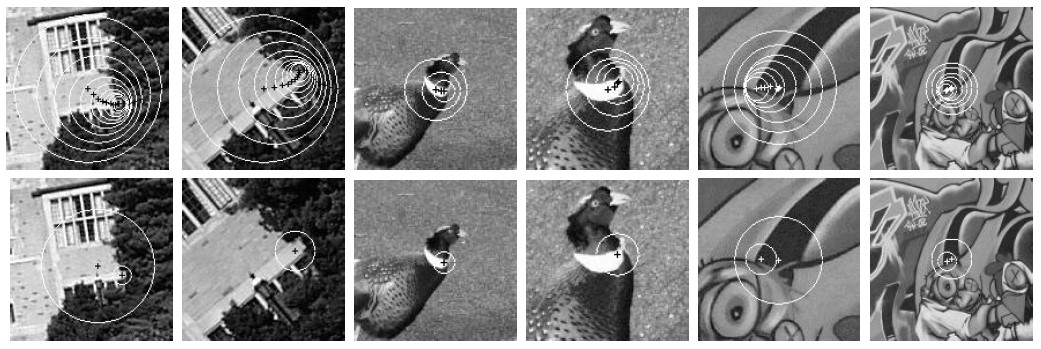
\includegraphics[width=0.8\textwidth]{gambar/Scale invariant interest point detection.jpg}
  \caption{}
\end{figure}

Pada gambar di atas kami menyajikan beberapa contoh titik yang terdeteksi dengan metode Harris-Laplace. Baris atas menunjukkan titik yang terdeteksi dengan detektor Harris multiskala. Skala deteksi diwakili oleh lingkaran di sekitar titik dengan radius \(3\sigma_{I}\) . Perhatikan, bagaimana titik minat, yang terdeteksi untuk struktur gambar yang sama, mengubah lokasinya dalam arah gradien relatif terhadap skala deteksi. Seseorang dapat menentukan rantai poin dan memilih hanya satu dari mereka untuk mewakili struktur lokal. Titik serupa terletak di lingkungan kecil dan dapat ditentukan dengan membandingkan deskriptornya. Namun, untuk struktur lokal yang ada dalam berbagai skala, konten informasi dapat berubah. Dalam pendekatan, ukuran LoG digunakan untuk memilih titik representatif untuk struktur tersebut. Selain itu, Laplacian memungkinkan titik-titik karakteristik yang sesuai untuk dipilih (baris bawah) bahkan jika transformasi antar citra signifikan. Kadang-kadang, dua atau lebih titik dipilih, tetapi tanpa pengetahuan sebelumnya tentang perubahan skala antara gambar, harus menyimpan semua titik yang dipilih. Lokasi dan skala titik-titik benar sehubungan dengan transformasi antar gambar.

\begin{figure}
  \centering{}
  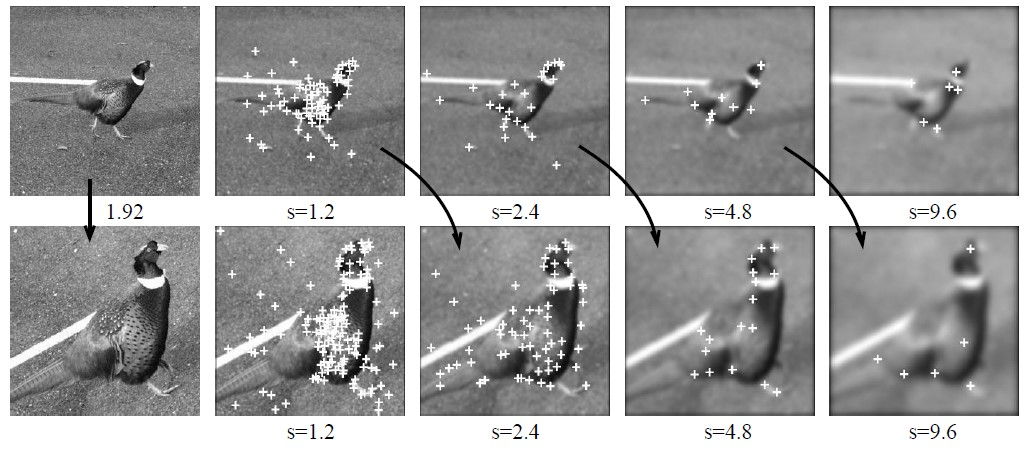
\includegraphics[width=0.8\textwidth]{gambar/Point detect.jpg}
  \caption{}
\end{figure}

Gambar di atas menunjukkan representasi skala-ruang untuk dua citra dengan titik-titik yang dideteksi dengan metode Harris-Laplace. Untuk setiap level skala objek, kami menyajikan titik-titik yang dipilih. Ada banyak korespondensi point-to-point antara level yang rasio skalanya sesuai dengan perubahan skala nyata antara gambar (ditunjukkan dengan pointer). Selain itu, sangat sedikit titik yang terdeteksi di lokasi yang sama tetapi pada level yang berbeda. Oleh karena itu, titik-titik merupakan karakteristik pada bidang citra dan dalam dimensi skala.

\section{\textbf{Affine invariant detector}}
Sebuah detektor invarian affine dapat dilihat sebagai generalisasi dari detektor invarian skala. Dalam kasus transformasi affine penskalaan bisa tidak seragam, yang berbeda di setiap arah. Penskalaan yang tidak seragam berpengaruh terhadap lokalisasi, skala dan bentuk struktur lokal yang khas. Oleh karena itu, detektor skala invarian gagal dalam kasus transformasi affine yang signifikan.

\subsection{\textbf{Harris-Affine detector}}
Dalam kasus transformasi afin, perubahan skala dapat berbeda di setiap arah. Detektor Harris-Laplace yang disajikan akan gagal dalam kasus transformasi affine yang penting karena mengasumsikan perubahan skala yang seragam. Angka ?? menyajikan dua pasang titik yang terdeteksi dalam gambar dengan deformasi afin yang signifikan. Baris atas menunjukkan titik yang terdeteksi dengan detektor Harris multiskala. Skala yang dipilih dengan Laplacian ditampilkan dalam warna hitam. Jika diproyeksikan lingkungan lingkaran dari titik yang bersesuaian menggunakan transformasi affine, diperoleh daerah elips yang tidak menutupi bagian yang sama dari gambar. Dapat dilihat titik yang diproyeksikan ditampilkan di baris bawah (berwarna putih) ditumpangkan pada titik Harris-Laplace yang sesuai (berwarna hitam)

\begin{figure}
  \centering{}
  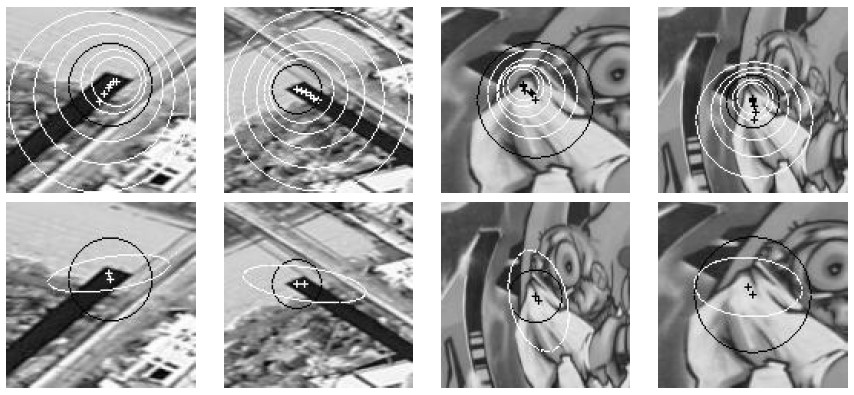
\includegraphics[width=0.8\textwidth]{gambar/Non Adapted interest point.jpg}
  \caption{}
\end{figure}

Dalam kasus transformasi halus, ketika perubahan skala tidak selalu sama di setiap arah, skala yang dipilih secara otomatis tidak mencerminkan transformasi sebenarnya dari suatu titik. Diketahui bahwa Harris maxima lokal mengubah lokasi spasial sehubungan dengan skala deteksi. Dengan demikian, kesalahan tambahan terjadi pada lokasi titik jika skala deteksi tidak sesuai dengan faktor skala antara pola gambar yang sesuai. Skala deteksi dalam arah ortogonal harus bervariasi secara independen, untuk menangani kemungkinan penskalaan afine. Misalkan kedua skala dapat disesuaikan dengan struktur gambar lokal. Oleh karena itu, kita menghadapi masalah komputasi matriks momen kedua dalam ruang skala affine Gaussian, di mana lingkungan titik lingkaran digantikan oleh elips.

Banyak hasil yang sukses dalam memperkirakan deformasi afin dengan matriks momen kedua membuktikan kegunaan matriks ini. Telah mengeksplorasi propertinya untuk memilih skala deteksi. Properti yang memadai dijelaskan di bagian 2.1.3. Untuk titik tertentu \(x\) matriks momen kedua \(\mu \) dalam ruang skala tidak seragam didefinisikan oleh:

\begin{equation*}
  \mu(x,\Sigma_{I},\Sigma_{D}) = g(\Sigma_{I}) * ((\nabla L)(x,\Sigma_{D})(\nabla L)(x,\Sigma_{D})^{T})
\end{equation*}

di mana \(\Sigma_{I}\) dan \(\Sigma_{D}\) adalah matriks kovarians yang menentukan integrasi dan diferensiasi kernel Gaussian. Untuk mengurangi ruang pencarian, diberlakukan kondisi \(\Sigma_{I}=s\Sigma_{D}\), dimana \(s\) adalah skalar. Selanjutnya, untuk membatasi ruang pencarian inisialisasi detektor affine dengan interest point diekstrak oleh detektor Harris multi-skala. Detektor apa pun dapat digunakan untuk menentukan lokalisasi spasial dari titik awal, tetapi detektor Harris juga didasarkan pada \emph{Second moment matrix}, agar cocok secara alami dalam kerangka kerja ini. Untuk mendapatkan matriks bentuk untuk setiap titik kepentingan menghitung deskriptor momen kedua dengan skala integrasi dan diferensiasi yang dipilih secara otomatis. Garis besar metode deteksi kami disajikan dalam berikut

\begin{enumerate}
  \item lokalisasi spasial dari suatu titik perhatian pada skala dan bentuk tertentu ditentukan oleh maksimum lokal dari fungsi Harris,
  \item skala integrasi dipilih pada skala ekstrim dari turunan yang dinormalisasi,
  \item skala diferensiasi dipilih pada maksimum isotropi yang dinormalisasi,
  \item matriks adaptasi bentuk menormalkan lingkungan titik.
\end{enumerate}

Berikut ini dibahas secara rinci setiap langkah dari algoritma.

\textbf{Shape adaptation matrix.} metode adaptasi bentuk iteratif bekerja pada domain citra yang ditransformasikan. Seperti yang disajikan di bagian 2.1, alih-alih menerapkan kernel affine Gaussian, kami mengubah gambar dan menerapkan kernel yang seragam. Itu memungkinkan penggunaan implementasi rekursif filter Gaussian seragam untuk menghitung \(L_{x}\) dan \(L_{y}\). Matriks momen kedua dihitung menurut persamaan ??. Jendela lokal \(W\) berpusat pada titik minat \(x\) dan ditransformasikan oleh matriks:

\begin{equation}
  U^{k-1} = (\mu^{-\frac{1}{2}})^{k-1} \cdot (\mu^{-\frac{1}{2}})^{1} \dots U^{0}
\end{equation}

dalam langkah \((k)\) dari algoritma iteratif. 
Berikut ini kami menyebut operasi ini sebagai transformasi-U. Perhatikan, bahwa matriks \(\mu\) 
baru dihitung pada setiap iterasi dan matriks U adalah gabungan dari akar kuadrat dari matriks momen kedua. 
Kami memastikan bahwa gambar asli diambil sampelnya dengan benar dengan menyetel nilai eigen yang lebih besar \(\lambda_{max}(U)=1\). Ini berarti patch gambar diperbesar ke arah \(\lambda_{min}(U)\). Untuk titik tertentu integrasi dan skala lokal menentukan matriks momen kedua \(\mu\). Parameter skala ini secara otomatis terdeteksi di setiap langkah iterasi. Dengan demikian, matriks \(\mu\) yang dihasilkan tidak bergantung pada skala awal dan resolusi gambar.

\textbf{Integration scale} Untuk titik spasial tertentu, kami secara otomatis memilih skala karakteristiknya. Untuk mempertahankan invarian terhadap perubahan ukuran, kami memilih skala integrasi \(\sigma_{I}\) di mana Laplacian yang dinormalisasi mencapai skala maksimum lokal. Dalam kasus perubahan skala yang lemah, cukup menjaga \(\sigma_{I}\) konstan selama iterasi. Di hadapan deformasi afin penting perubahan skala sangat berbeda di setiap arah. Dengan demikian, skala karakteristik yang terdeteksi pada gambar asli dan versi transformasi U-nya dapat berbeda secara signifikan. Oleh karena itu, sangat penting untuk memilih skala integrasi setelah menerapkan transformasi U. Kami menggunakan prosedur yang mirip dengan yang dijelaskan untuk versi perluasan detektor Harris-Laplace, di bagian 2.3.1. Hal ini memungkinkan titik-titik awal menyatu menuju titik di mana skala dan matriks momen kedua tidak berubah lagi. Perhatikan, bahwa skala ekstrem harus memiliki jenis yang sama selama iterasi. Jika tidak, metode dapat beralih antara maksimum dan minimum jika terdapat kedua jenis ekstrem dalam rentang skala yang dipindai.

\textbf{Differentiation scale} Skala diferensiasi lokal kurang kritis dan dapat diatur secara proporsional dengan skala 
integrasi \(\sigma_{D} = s \sigma_{I}\) , dimana \(s\) adalah faktor konstan. Namun, kami mengusulkan untuk mendasarkan skala 
turunan pada ukuran isotropi yang diperkenalkan dibagian 2.1.3. Faktor \(s\) umumnya dipilih dari rentang \([0.5, \cdot , 0.7]\). 
Solusinya adalah memilih skala diferensiasi yang isotropi lokalnya diasumsikan maksimum pada rentang skala ini. 
Mengingat skala integrasi \(\sigma_{I}\) kami memilih \(s \in [0.5,\cdot,0.7]\) dimana ukuran \(Q\) mengasumsikan maksimum. 
Solusi ini dimotivasi oleh fakta bahwa skala lokal memiliki pengaruh penting pada konvergensi matriks momen kedua. 
Prosedur iteratif konvergen menuju matriks dengan nilai eigen yang sama. Semakin kecil perbedaan antara nilai eigen \(\lambda_{max}(\mu),\lambda_{min}(\mu)\) 
dari matriks awal, semakin dekat solusi akhir dan prosedur semakin cepat konvergen. Perhatikan bahwa ukuran Harris sudah memilih titik dengan dua nilai eigen 
besar. Perbedaan besar antara nilai eigen menyebabkan penskalaan besar dalam satu arah oleh transformasi U. 
Intinya tidak konvergen ke solusi yang stabil karena kebisingan. Pemilihan skala lokal memungkinkan diperoleh 
rasio nilai eigen yang masuk akal dan titik-titik konvergen, yang tidak akan konvergen jika rasionya terlalu besar.

\textbf{Spatial localization} telah menunjukkan bagaimana maxima lokal dari ukuran Harris ubah lokasinya jika skala deteksi berubah. 
Bisa juga mengamati efek ini, ketika perubahan skala berbeda di setiap arah. Deteksi dengan skala yang berbeda dalam arah x dan y diganti dengan mengadaptasi gambar dan kemudian menerapkan skala yang sama di kedua arah. Normalisasi affine dari suatu lingkungan titik sedikit menggeser maksima spasial dari fungsi Harris. Akibatnya, kami mendeteksi ulang maksimum di jendela normalisasi affine W . Dengan demikian, kami memperoleh vektor perpindahan ke maksimum terdekat dalam domain gambar yang dinormalisasi-U. Lokasi titik awal dikoreksi 
dengan vektor perpindahan yang ditransformasikan kembali ke domain gambar asli:

\begin{equation*}
  x^{k} = x^{k-1} + U^{k-1} \dots (x_{w}^{k} - x_{w-1}^{k-1})
\end{equation*}

dimana \(x_{w}\) adalah titik di koordinat gambar yang diubah-U.

\textbf{Convergence criterion.} Bagian penting dari prosedur iterasi adalah kriteria penghentian. 
Ukuran konvergensi dapat didasarkan pada matriks U atau \(\mu\). Jika kriteria didasarkan pada \(\mu\) yang 
dihitung dalam setiap langkah iterasi, kami mensyaratkan matriks ini cukup dekat dengan rotasi murni. 
Ini menyiratkan bahwa \(\lambda_{max}(\mu)\) dan \(\lambda_{min}(\mu)\) adalah sama. 
Dalam praktiknya kami mengizinkan kesalahan kecil \(e_{C}=0.05\).

\begin{equation}
  \frac{\lambda_{max}(\mu)-\lambda_{min}(\mu)}{\lambda_{max}(\mu)} < \epsilon_{C}
\end{equation}

Kemungkinan lain adalah menguraikan matriks \(U = R^{T}.D.R\) menjadi rotasi \(R\) dan penskalaan \(D\) dan membandingkan 
transformasi yang berurutan. Kami mengizinkan titik jika transformasi \(R\) dan \(D\) berturut-turut cukup mirip. 
Kedua kriteria terminasi tersebut memberikan hasil akhir yang sama. Poin penting lainnya adalah menghentikan iterasi jika 
terjadi divergensi. Dalam teori ada kasus tunggal ketika rasio nilai eigen cenderung tak terhingga. 
Oleh karena itu, titik tersebut harus ditolak jika rasionya terlalu besar (yaitu \(e_{I}\) = 6), 
jika tidak maka akan menyebabkan struktur memanjang yang tidak stabil.

\begin{equation}
  \frac{\lambda_{max}(D)}{\lambda_{min}(D)} > \epsilon_{\iota}
\end{equation}

Properti konvergensi dari algoritma adaptasi bentuk dipelajari secara ekstensif. Terlihat bahwa selain kasus tunggal, titik konvergensi selalu unik. Secara umum prosedur konvergen asalkan estimasi awal deformasi affine cukup dekat dengan deformasi yang sebenarnya dan skala integrasi dipilih dengan benar sehubungan dengan ukuran struktur gambar lokal.

\textbf{Detection algorithm}mengusulkan prosedur iteratif yang memungkinkan titik-titik awal untuk bertemu dengan titik-titik kovarian affine, yaitu titik-titik yang secara kovarian berubah dengan sudut pandang. Untuk menginisialisasi algoritme kami, kami menggunakan poin yang diekstraksi oleh detektor Harris multi-skala. Titik-titik ini tidak terdeteksi dengan cara invarian affine karena kernel Gaussian yang tidak diadaptasi, tetapi memberikan perkiraan lokalisasi dan skala untuk pencarian lebih lanjut untuk titik minat kovarian affine. 
Untuk titik minat awal tertentu \(x^{(0)}\) kami menerapkan prosedur berikut:

\begin{enumerate}
  \item menginisialisasi \(U^(0)\) ke matriks identitas,
  \item menormalkan jendela \(W(x_{w})=I(x)\) berpusat di \(U^{(k-1)}x_{w}^{(k-1)} = x^{(k-1)}\),
  \item pilih skala integrasi \(\sigma_{I}\) dalam \(x^{(k-1)}_{w}\),
  \item pilih skala diferensiasi \(\sigma_{D}=s\sigma_{I}\), yang memaksimalkan \(\frac{\lambda_{min}(\mu)}{\lambda_{max}(\mu)}\) dengan \(s \in [0.5,\cdot,0.7]\) dan \(\mu = \mu(x_{w}^{(k-1)}),\sigma_{D},\sigma_{I}\)
  \item mendeteksi lokalisasi spasial \(x^{(k)}_{w}\) dari maksimum ukuran Harris terdekat dengan \(x^{(k-1)}_{w}\) dan hitung lokasi titik minat \(x^{(k-1)}_{w}\)
  \item menghitung \(\mu^{(k)}_{i}=\mu^{-\frac{1}{2}}(x^{(k)}_{w},\sigma_{D},\sigma_{I})\)
  \item transformasi gabungan \(U^{(k)}=\mu^{-\frac{1}{2}}U^{(k-1)}\) dan normalisasi \(U^{(k)}\) ke \(\lambda_{max}(U^{(k)})=1\)
  \item lanjut ke langkah 2 jika \(1 - \frac{\lambda_{min}(\mu^{k}_{i})}{\lambda_{max}(\mu^{(k)}_{i})} > e_{C}\)
\end{enumerate}

\begin{figure}
  \centering{}
  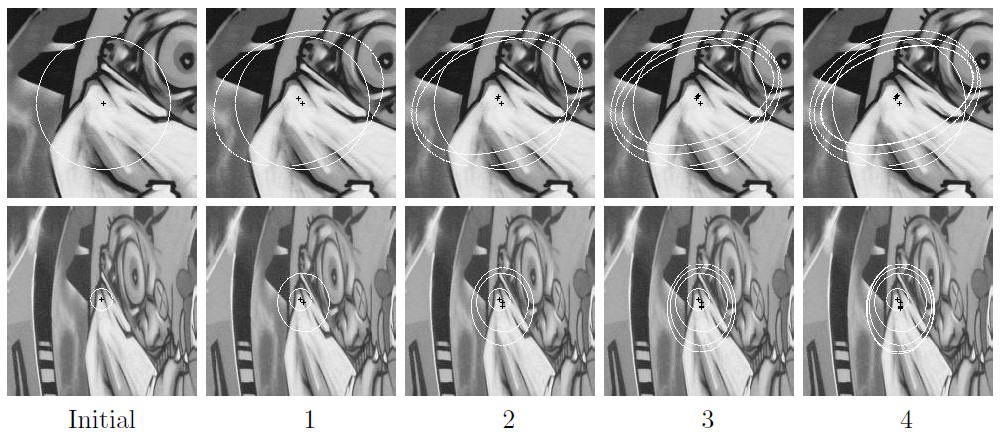
\includegraphics[width=0.8\textwidth]{gambar/Iterative evolution.jpg}
  \caption{}
\end{figure}

Meskipun perhitungan mungkin tampak sangat memakan waktu, perhatikan bahwa sebagian besar waktu dihabiskan untuk menghitung Lx dan Ly , yang dilakukan hanya sekali dalam setiap langkah jika hubungan antara integrasi dan skala lokal konstan. Perulangan iterasi dimulai dengan memilih skala integrasi karena kami menyadari bahwa bagian algoritme ini paling kuat untuk kesalahan pelokalan kecil dari suatu titik minat. Namun, skala \(\sigma_{I}\) berubah jika bentuk tambalan diubah. Diberikan solusi perkiraan awal, algoritme yang disajikan memungkinkan seseorang untuk secara iteratif memodifikasi bentuk, skala, dan lokasi spasial suatu titik dan menyatu dengan struktur lokal, yang ditentukan meskipun transformasi afin berubah-ubah. Gambar 10 menunjukkan titik-titik afin yang terdeteksi dalam langkah-langkah berurutan dari prosedur berulang. Setelah iterasi keempat lokasi, skala dan bentuk titik tidak berubah lagi. Kita dapat melihat bahwa elips menutupi wilayah gambar yang sama meskipun terjadi deformasi affine yang kuat.

\textbf{Selection of similar affine points} Asalkan wilayah yang dinormalisasi adalah isotropik, ada satu maksimum spasial dari ukuran Harris dan satu skala karakteristik untuk struktur 
lokal yang dipertimbangkan. Oleh karena itu, beberapa titik awal yang berkorespondensi dengan fitur yang sama 
tetapi terdeteksi pada level skala yang berbeda dapat menyatu menuju satu lokasi dan skala titik. Sangat mudah untuk mengidentifikasi titik-titik ini dengan membandingkan 
lokasinya \((x,y)\), skala \(\sigma_{I}\) , regangkan \(\lambda_{min}(U)\) dan miring. Kemiringan dipulihkan dari matriks rotasi R, di mana \(U=R^{T}.D.R\) Kami mendefinisikan titik serupa jika masing-masing parameter ini cukup dekatdengan parameter titik referensi. Terakhir, kami menghitung parameter rata-rata dan memilih titik yang paling mirip dari kumpulan titik yang diidentifikasi. Sebagai hasilnya, untuk citra tertentu kita memperoleh sekumpulan titik, di mana masing-masing mewakili lokasi dan struktur citra yang berbeda.

\subsection{\textbf{Affine covariant points}}

\begin{figure}
  \centering{}
  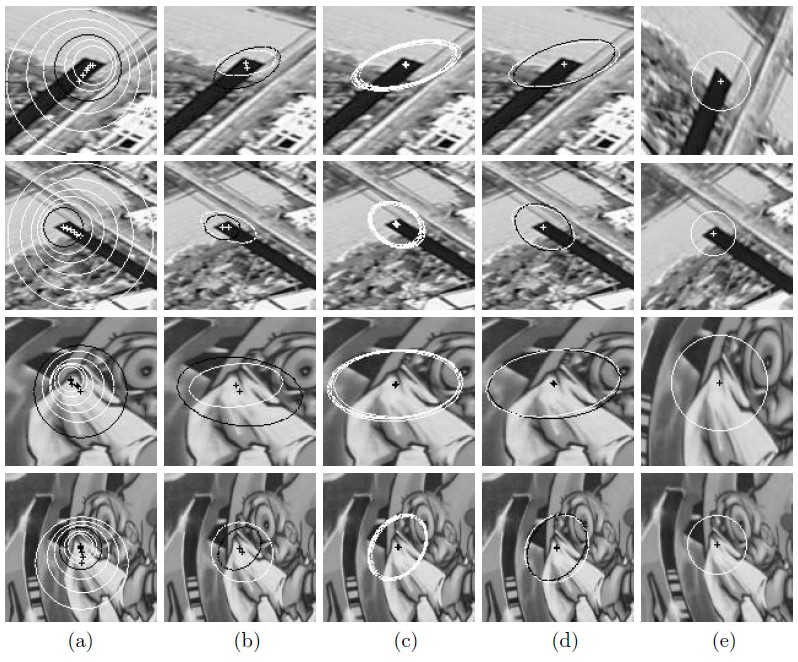
\includegraphics[width=0.8\textwidth]{gambar/Affine invariant interest point detection.jpg}
  \caption{}
\end{figure}

Gambar di atas menyajikan dua contoh karakteristik struktur lokal. Kolom (a) ditampilkan 
titik yang digunakan untuk inisialisasi, yang dideteksi oleh detektor Harris multi-skala.
Lingkaran di sekitar titik menunjukkan skala pendeteksian, di mana jari-jari lingkaran adalah \(3\sigma_{I}\) Lingkaran berwarna hitam menunjukkan
titik yang dipilih oleh detektor Harris-Laplace. Perhatikan bahwa ada perpindahan penting antara titik yang terdeteksi pada skala yang berbeda dan lingkaran pada gambar yang sesuai (baris atas dan bawah) tidak menutupi bagian gambar yang sama. Pada kolom (b) kami menunjukkan titik-titik (berwarna hitam) yang terdeteksi dengan menerapkan prosedur iteratif pada titik-titik Harris-Laplace. Skala dan lokasi titik konstan selama iterasi. Wilayah terkait yang diproyeksikan ditampilkan dalam warna putih dan dengan jelas menunjukkan perbedaan dalam lokalisasi dan bentuk wilayah. Skala awal tidak terdeteksi dengan benar karena operator Laplacian yang tidak diadaptasi secara seragam. Demikian pula, lokasi titik berbeda dalam 3-4 piksel. Dalam pendekatan kami, titik-titik yang sesuai dengan struktur fisik yang sama, tetapi terdeteksi di lokasi yang berbeda karena skala, menyatu ke lokasi titik yang sama. Oleh karena itu, jumlah poin bunga efektif berkurang. Titik-titik kovarian affine, tempat titik-titik awal bertemu disajikan dalam kolom (c). Poin-poin ini diperoleh dengan menerapkan algoritme yang dijelaskan di bagian sebelumnya. Kita dapat melihat bahwa metode konvergen dengan benar meskipun lokasi dan skalanya
titik awal relatif jauh dari titik konvergensi. Konvergensi pada umumnya diperoleh dalam waktu kurang dari 10 iterasi. Perbedaan kecil antara daerah di kolom (d) disebabkan oleh ketidaktepatan estimasi skala dan kesalahan \(e_{C}\). Kolom (e) menunjukkan titik "rata-rata" yang dinormalisasi
dengan perkiraan matriks untuk menghilangkan peregangan dan kemiringan. Kita dapat melihat dengan jelas bahwa wilayah berkorespondensi antara dua gambar (baris atas dan bawah).
%!TEX root = ./template-skripsi.tex
%-------------------------------------------------------------------------------
%                            	BAB III
%               		    METODE PENELITIAN
%-------------------------------------------------------------------------------

\chapter{Metode Penelitian}

\section{Flow Penelitian}

\begin{figure}
  \centering{}
  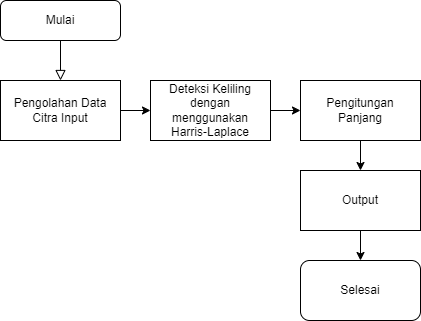
\includegraphics[width=0.45\textwidth]{gambar/Flowchart Penelitian.png}
  \caption{Diagram Penghitungan panjang ikan}
\end{figure}

\begin{figure}
  \centering{}
  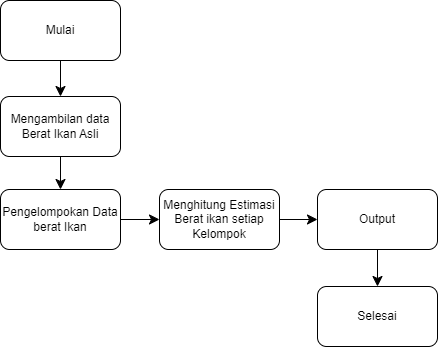
\includegraphics[width=0.45\textwidth]{gambar/Penghitungan Berat.png}
  \caption{Diagram Penghitungan berat ikan}
\end{figure}

\section{Deskripsi Sistem}

Dalam Penelitian yang akan dibuat adalah sebuah sistem yang dapat menghitung panjang serta berat rata-rata dari se-ekor ikan dengan menggunakan metode \emph{Harris-Corrner}.
Fokus dari penulis terhadap penelitian ini adalah untuk menghitung panjang serta berat rata-rata dari objek ikan. 
Citra yang digunakan oleh penulis diambil dari sebuah peternakan ikan, dimana citra tersebut akan penulis gunakan dalam pengujian sistem penghitungan panjang serta berat rata-rata ikan.

Bahasa yang penulis gunakan dalam perancangan sistem adalah Python 3. 
Tujuan penelitian adalah mendapatkan hasil perhitungan panjang dan berat ikan secara komputasi yang mana dihasilkan panjang dan berat ikan dari sebuah citra ikan. 

Tahapan yang akan diproses dalam penghitungan berat dan panjang ikan dengan menggunakan \emph{Harris-corner} adalah memasukan atau menginput citra ikan, lalu mendeteksi korner dari ikan menggunakan \emph{Harris-corner} dan menghitung panjang serta berat ikan mengunakan korner hasil dari \emph{Harris-corner}. 




% %!TEX root = ./template-skripsi.tex
%-------------------------------------------------------------------------------
%                            	BAB IV
%               		KESIMPULAN DAN SARAN
%-------------------------------------------------------------------------------

\chapter{UJI COBA DAN HASIL UJI COBA}

\section{Uji Coba}
Uji coba sistem dilakukan terhadap 30 responden anggota KOPMA UNJ dengan rincian, \textit{admin} yang terdiri dari 2 responden, pengawas yang terdiri dari 3 responden, dan anggota yang terdiri dari 25 responden. Setiap responden akan melakukan uji coba terhadap sistem yang dibuat berdasarkan peran masing-masing responden. Uji coba yang dilakukan menggunakan data dari hasil sebaran kuesioner \textit{User Acceptance Test}. \textit{User Acceptance Test} bertujuan untuk mengetahui perihal sistem yang dikembangkan apakah sudah sesuai dengan kebutuhan \textit{user} atau belum. Skala yang digunakan dalam penelitian ini adalah skala \textit{likert}.

Langkah-langkah pengujian sistem informasi Koperasi Mahasiswa Universitas Negeri Jakarta yang akan dilakukan adalah sebagai berikut:
\begin{enumerate}
	\item \textit{User} melakukan pendaftaran anggota.
	\item \textit{Admin} melakukan verifikasi penerimaan anggota.
	\item \textit Seluruh \textit{user} dapat mengelola biodata pribadi.
	\item \textit{Admin} mengelola status keanggotaan setiap \textit{user} (\textit{admin}, pengawas, atau anggota biasa).
	\item Anggota dan pengawas yang sudah memiliki akun dapat mengakses ke dalam sistem sesuai berandanya masing-masing.
	\item \textit{Admin} menambahkan data barang, stok, simpanan, transaksi anggota, dan keuangan.
	\item Data yang \textit{admin} tambahkan akan muncul dan dapat dilihat di beranda semua \textit{user}.
	\item \textit{Admin} mengelola (sunting dan hapus) data barang, stok, simpanan, transaksi anggota, dan keuangan.
	\item Data yang \textit{admin} kelola akan berubah dan dapat dilihat di beranda semua \textit{user}.	
	\item Pengawas menambahkan data penilaian untuk KOPMA UNJ.
	\item Data yang pengawas tambahkan akan muncul dan dapat dilihat di beranda  semua \textit{user}.
	\item Pengawas mengelola (sunting dan hapus) data penilaian untuk KOPMA UNJ.
	\item Data yang pengawas kelola akan berubah dan dapat dilihat di beranda semua \textit{user}.	
\end{enumerate}

Fitur milik setiap \textit{user} yang akan diuji pada sistem informasi Koperasi Mahasiswa Universitas Negeri Jakarta adalah sebagai berikut:

\begin{itemize}
	\item \textit{Admin}
	\begin{enumerate}
		\item Masuk ke dalam sistem
		\item Penyuntingan data pribadi
		\item Pengelolaan anggota (tambah, kesesuaian \textit{id}, detail, pemutihan, sunting, \textit{reset password}, tambah periode, pengelompokan, pemulihan, keuangan anggota, dan cetak)
		\item Pengelolaan barang (tambah, sunting, hapus, cetak, dan pengelompokan)
		\item Pengelolaan stok (tambah, hapus, dan cetak)
		\item Pengelolaan simpanan (tambah, hapus, cetak, dan pengelompokan)
		\item Pengelolaan transaksi (tambah, hapus, dan cetak)
		\item Transparansi penilaian
		\item Pengelolaan dan kesesuaian arus keuangan (tambah dana tambahan dan beban lain)
		\item Pengelolaan \textit{admin} (tambah dan hapus \textit{admin})
		\item Pengelolaan pengawas (tambah dan hapus pengawas)
		\item Pengelolaan penerimaan anggota (terima dan tolak anggota)
		\item Keluar dari sistem
	\end{enumerate}

	\item Anggota
	\begin{enumerate}
		\item Melakukan pendaftaran
		\item Masuk ke dalam sistem
		\item Penyuntingan data pribadi
		\item Transparansi data (barang, stok, transaksi, penilaian, dan arus keuangan)
		\item Keluar dari sistem
	\end{enumerate}
	
	\item Pengawas
	\begin{enumerate}
		\item Masuk ke dalam sistem
		\item Penyuntingan data pribadi
		\item Transparansi data (barang, stok, transaksi, dan arus keuangan)
		\item Pengelolaan penilaian (tambah, sunting, hapus, dan cetak)
		\item Keluar dari sistem
		\end{enumerate}
	\end{itemize}

Semua fitur yang diuji memiliki penilaian yang dirincikan menjadi beberapa kategori. Data kuantitatif akan dianalisis dengan menggunakan skala \textit{ likert}. Berikut kategori dan skor penilaian dalam tahap pengujian\textit{ User Acceptance Test} pada sistem informasi Koperasi Mahasiswa Universitas Negeri Jakarta dengan menggunakan skala \textit{likert}:\\

\begin{tabular}{lll}
SS& = Sangat Setuju& diberikan nilai 5\\
S& = Setuju& diberikan nilai 4\\
C& = Cukup& diberikan nilai 3\\
TS& = Tidak Setuju& diberikan nilai 2\\
STS& = Sangat Tidak Setuju& diberikan nilai 1\\
\\
\end{tabular}

Kemudian hasil pendataan yang telah didapatkan dengan teknik penyebaran angket dikalkulasikan dengan menggunakan sistem penilaian sebagai berikut:

\begin{itemize}
	\item Nilai total
	
	Nilai total merupakan nilai dari hasil perhitungan antara responden kuesioner angket dengan nilai di setiap poin pertanyaan. Berikut merupakan rumus nilai total:
	
	\textit{Nilai total = jumlah nilai setiap soal}
	
	\item Nilai rata-rata
	
	Nilai rata-rata merupakan nilai dari hasil perhitungan antara nilai total dengan jumlah responden yang mengisi kuesioner angket. Berikut merupakan rumus dari nilai rata-rata:

	\textit{Nilai rata-rata = nilai total / jumlah responden}
	
\end{itemize}

Untuk mengetahui kualitas produk yang dikembangkan layak atau tidak, maka perlu ditentukan dengan menghitung seluruh nilai rata-rata dari setiap pertanyaan. Nilai tersebut kemudian akan dibandingkan dengan interpretasi skor pada skala \textit{likert}. Analisis data yang disajikan ke distribusi skor dan persentase terhadap kategori menggunakan interpretasi skor untuk skala \textit{likert}. Berikut rentang interpretasi skor untuk skala \textit{likert}:\\

\begin{tabular}{lll}
	Nilai& = 0\% - 20\%& Sangat Kurang Sesuai \\
	Nilai& = 21\% - 40\%& Kurang Sesuai\\
	Nilai& = 41\% - 60\%& Cukup Sesuai\\
	Nilai& = 61\% - 80\%& Sesuai\\
	Nilai& = 81\% - 100\%& Sangat Sesuai\\
\end{tabular}

\section{Hasil Uji Coba}
Berdasarkan hasil uji coba \textit{User Acceptance Test} yang dilakukan terhadap 30 anggota KOPMA UNJ, yakni \textit{admin} yang terdiri dari 2 responden, pengawas terdiri dari 3 responden, dan anggota terdiri dari 25 responden, diperoleh hasil uji coba sebagai berikut:

\subsection{\textit{Admin}}
Berikut merupakan daftar pertanyaan \textit{User Acceptance Test} pada \textit{Admin}:

\begin{table}[H]
	\centering
	\caption{Daftar Pertanyaan \textit{User Acceptance Test} pada \textit{Admin}}
	\includegraphics[width=1.0\textwidth]{gambar/Tabel_Admin1}
\end{table}

\begin{table}[H]
	\centering
	\caption{Daftar Pertanyaan \textit{User Acceptance Test} pada \textit{Admin}}
	\includegraphics[width=1.0\textwidth]{gambar/Tabel_Admin2}
\end{table}

Setelah kuisioner \textit{admin} diberikan kepada responden, kemudian data kuesioner diolah untuk mendapatkan hasil penilaian \textit{user acceptance test}. Adapun hasil penilaian \textit{user acceptance test} tersebut yaitu:

\begin{table}[H]
	\centering
	\caption{Data Hasil Penyebaran Kuesioner \textit{User Acceptance Test} pada \textit{Admin}}
	\includegraphics[width=1\textwidth]{gambar/Hasil_Admin}
\end{table}

Dari hasil penilaian pengujian \textit{user acceptance test} dapat diambil kesimpulan yaitu:

\begin{enumerate}
	\item Pengguna sistem yang telah memilih Sangat Tidak Setuju (STS) memiliki persentase 0\%
	\item Pengguna sistem yang telah memilih Tidak Setuju (TS) memiliki persentase 0\%
	\item Pengguna sistem yang telah memilih Cukup (C) memiliki persentase 8\%.
	\item Pengguna sistem yang telah memilih Setuju (S) memiliki persentase 57\%.
	\item Pengguna sistem yang telah memilih Sangat Setuju (SS) memiliki persentase 35\%.
	\item Rata-rata penerimaan \textit{user} adalah 4,27 dari 5 atau sekitar 85\%.
\end{enumerate}

\begin{figure}[H]
	\centering
	\includegraphics[width=1\textwidth]{gambar/Grafik_Admin}
	\caption{Grafik Hasil Penyebaran Kuesioner \textit{User Acceptance Test} pada \textit{Admin}}
\end{figure}

Berdasarkan hasil pengujian \textit{user acceptance test} yang diujikan kepada 2 responden \textit{admin}, dapat dilihat bahwa secara keseluruhan 35\% menjawab sangat setuju, 57\% menjawab setuju, 8\% menjawab cukup, serta rata-rata penerimaan \textit{user} terhadap kesesuaian sistem dengan kebutuhan adalah 4,27 dari 5 atau sekitar 85\%, oleh karena itu dapat diambil kesimpulan bahwa fitur yang \textit{admin} butuhkan dalam sistem informasi yang dirancang sudah sangat sesuai dengan kebutuhan dan berjalan dengan baik.  

\subsection{\textit{Anggota}}
Berikut merupakan daftar pertanyaan \textit{User Acceptance Test} pada Anggota

\begin{table}[H]
	\centering
	\caption{Daftar Pertanyaan \textit{User Acceptance Test} pada Anggota}
	\includegraphics[width=1\textwidth]{gambar/Tabel_Anggota}
\end{table}

Setelah kuisioner anggota diberikan kepada responden, kemudian data kuesioner diolah untuk mendapatkan hasil penilaian \textit{user acceptance test}. Adapun hasil penilaian \textit{user acceptance test} tersebut yaitu:

\begin{table}[H]
	\centering
	\caption{Data Hasil Penyebaran Kuesioner \textit{User Acceptance Test} pada Anggota}
	\includegraphics[width=1\textwidth]{gambar/Hasil_Anggota}
\end{table}

Dari hasil pengujian \textit{user acceptance test} dapat diambil kesimpulan yaitu:

\begin{enumerate}
	\item Pengguna sistem yang telah memilih Sangat Tidak Setuju (STS) memiliki persentase 0\%
	\item Pengguna sistem yang telah memilih Tidak Setuju (TS) memiliki persentase 0\%
	\item Pengguna sistem yang telah memilih Cukup (C) memiliki persentase 23\%.
	\item Pengguna sistem yang telah memilih Setuju (S) memiliki persentase 58\%.
	\item Pengguna sistem yang telah memilih Sangat Setuju (SS) memiliki persentase 19\%.
	\item Rata-rata penerimaan \textit{user} adalah 3,96 dari 5 atau sekitar 79\%.
\end{enumerate}

\begin{figure}[H]
	\centering
	\includegraphics[width=1\textwidth]{gambar/Grafik_Anggota}
	\caption{Grafik Hasil Penyebaran Kuesioner \textit{User Acceptance Test} pada Anggota}
\end{figure}

Berdasarkan hasil pengujian \textit{user acceptance test} yang diujikan kepada 25 responden anggota, dapat dilihat bahwa secara keseluruhan 19\% menjawab sangat setuju, 58\% menjawab setuju, 23\% menjawab cukup, serta rata-rata penerimaan \textit{user} terhadap kesesuaian sistem dengan kebutuhan adalah 3,96 dari 5 atau sekitar 79\%, oleh karena itu dapat diambil kesimpulan bahwa fitur yang anggota butuhkan dalam sistem informasi yang dirancang sudah sesuai dengan kebutuhan dan berjalan dengan baik. 
\\
\\
\\
\\
\\

\subsection{\textit{Pengawas}}
Berikut merupakan daftar pertanyaan \textit{User Acceptance Test} pada Pengawas

\begin{table}[H]
	\centering
	\caption{Daftar Pertanyaan \textit{User Acceptance Test} pada Pengawas}
	\includegraphics[width=1\textwidth]{gambar/Tabel_Pengawas}
\end{table}

Setelah kuisioner pengawas diberikan kepada responden, kemudian data kuesioner diolah untuk mendapatkan hasil penilaian \textit{user acceptance test}. Adapun hasil penilaian \textit{user acceptance test tersebut} tersebut yaitu:

\begin{table}[H]
	\centering
	\caption{Data Hasil Penyebaran Kuesioner \textit{User Acceptance Test} pada Pengawas}
	\includegraphics[width=1\textwidth]{gambar/Hasil_Pengawas}
\end{table}

Dari hasil penilaian pengujian \textit{user acceptance test} dapat diambil kesimpulan yaitu:

\begin{enumerate}
	\item Pengguna sistem yang telah memilih Sangat Tidak Setuju (STS) memiliki persentase 0\%
	\item Pengguna sistem yang telah memilih Tidak Setuju (TS) memiliki persentase 0\%
	\item Pengguna sistem yang telah memilih Cukup (C) memiliki persentase 2\%.
	\item Pengguna sistem yang telah memilih Setuju (S) memiliki persentase 42\%.
	\item Pengguna sistem yang telah memilih Sangat Setuju (SS) memiliki persentase 56\%.
	\item Rata-rata penerimaan \textit{user} adalah 4,53 dari 5 atau sekitar 91\%.
\end{enumerate}

\begin{figure}[H]
	\centering
	\includegraphics[width=1\textwidth]{gambar/Grafik_Pengawas}
	\caption{Grafik Hasil Penyebaran Kuesioner \textit{User Acceptance Test} pada Pengawas}
\end{figure}

Berdasarkan hasil pengujian \textit{user acceptance test} yang diujikan kepada 3 responden pengawas, dapat dilihat bahwa secara keseluruhan 56\% menjawab sangat setuju, 42\% menjawab setuju, 2\% menjawab cukup, serta rata-rata penerimaan \textit{user} terhadap kesesuaian sistem dengan kebutuhan adalah 4,53 dari 5 atau sekitar 91\%, oleh karena itu dapat diambil kesimpulan bahwa fitur yang pengawas butuhkan dalam sistem informasi yang dirancang sudah sangat sesuai dengan kebutuhan dan berjalan dengan baik. 

% Baris ini digunakan untuk membantu dalam melakukan sitasi
% Karena diapit dengan comment, maka baris ini akan diabaikan
% oleh compiler LaTeX.
\begin{comment}
\bibliography{daftar-pustaka}
\end{comment}

% %!TEX root = ./template-skripsi.tex
%-------------------------------------------------------------------------------
%                            	BAB IV
%               		KESIMPULAN DAN SARAN
%-------------------------------------------------------------------------------

\chapter{KESIMPULAN DAN SARAN}

\section{Kesimpulan}
Berdasarkan hasil implementasi dan pengujian fitur sistem informasi yang telah dirancang, maka diperoleh kesimpulan sebagai berikut:

\begin{enumerate}
	\item Perancangan sistem informasi operasi serba usaha berbasis \emph{website} pada lembaga Koperasi Mahasiswa Universitas Negeri Jakarta menggunakan metode pengembangan perangkat lunak \textit{System Development Life Cycle} dengan \textit{spiral model} yang memiliki beberapa tahapan, yaitu analisis kebutuhan, perancangan desain sistem \textit{(prototype)}, pengimplementasian (\textit{coding \& testing-unit}), dan \textit{maintenance} (umpan balik dan tanggapan).
	
	\item Sistem informasi Koperasi Mahasiswa Universitas Negeri Jakarta dibangun dengan menggunakan \textit{framework codeigniter} dan \textit{framework bootstrap}. \textit{Codeigniter} untuk membangun sisi dalam \textit{back-end} dan \textit{Bootstrap} yang mempercantik bagian luar \textit{front-end}. Berdasarkan pengolahan data hasil kuesioner \textit{user acceptance test}, didapatkan rata-rata persentase mencapai angka 4,27 dari 5 atau sekitar 85\% untuk \textit{admin} yang berarti sistem sudah sangat sesuai, 3,96 dari 5 atau sekitar 79\% untuk anggota yang berarti sistem sudah sesuai, dan 4,53 dari 5 atau sekitar 91\% pada sistem pengawas yang berarti sistem sudah sangat sesuai.
	
	\item Sistem informasi Koperasi Mahasiswa Universitas Negeri Jakarta berbasis \textit{website} dibangun agar sistem pengelolaan data di KOPMA UNJ dapat menjadi lebih efektif dan efisian, serta agar kemungkinan adanya \textit{human error} dapat diatasi. Data yang dikelola berupa data anggota, barang, stok (pergudangan), simpanan, transaksi, penilaian, dan keuangan.
	
	\item Sistem informasi Koperasi Mahasiswa Universitas Negeri Jakarta berbasis \textit{website} mempermudah \textit{admin} dalam melakukan pengelolaan data yang ada di KOPMA UNJ, mempermudah pengawas dalam melakukan pengelolaan data penilan, dan membuat anggota dapat mengetahui transparansi simpanan yang mereka bayarkan hingga mengetahui transparansi sisa hasil usaha yang mereka dapatkan.
\end{enumerate}

\section{Saran}
Adapun saran untuk penelitian selanjutnya adalah:
\begin{enumerate} 
	\item Mengintegrasikan sistem informasi KOPMA UNJ dengan aplikasi dan sistem \textit{scanning barcode} agar proses transaksi semakin efektif dan efisien.
	\item Menambahkan dan mengintegrasikan sistem informasi KOPMA UNJ dengan aplikasi untuk \textit{scanning barcode} pada kartu anggota agar proses kebutuhan simpanan dan transaksi untuk anggota dapat semakin efektif dan efisien.
	\item Menambahkan sistem pengelolaan kegiatan keorganisasian KOPMA UNJ yang merupakan bagian dari peran KOPMA UNJ sebagai Organisasi Kemahasiswaan di UNJ.
	\item Membuat pengembangan sistem informasi KOPMA UNJ berbasis \textit{mobile} (\textit{android}).
\end{enumerate}


% Baris ini digunakan untuk membantu dalam melakukan sitasi
% Karena diapit dengan comment, maka baris ini akan diabaikan
% oleh compiler LaTeX.
\begin{comment}
\bibliography{daftar-pustaka}
\end{comment}


%-----------------------------------------------------------------
%Disini akhir masukan Bab
%-----------------------------------------------------------------


%-----------------------------------------------------------------
% Disini awal masukan untuk Daftar Pustaka
% - Daftar pustaka diambil dari file .bib yang ada pada folder ini
%   juga.
% - Untuk memudahkan dalam memanajemen dan menggenerate file .bib
%   gunakan reference manager seperti Mendeley, Zotero, EndNote,
%   dll.
%-----------------------------------------------------------------
% \bibliography{daftar-pustaka}
% \bibliographystyle{apalike}
\addcontentsline{toc}{chapter}{DAFTAR PUSTAKA}
\singlespacing{}
\printbibliography{}
%-----------------------------------------------------------------
%Disini akhir masukan Daftar Pustaka
%-----------------------------------------------------------------


\end{document}
